%%
%% This is file `sample-authordraft.tex',
%% generated with the docstrip utility.
%%
%% The original source files were:
%%
%% samples.dtx  (with options: `authordraft')
%% 
%% IMPORTANT NOTICE:
%% 
%% For the copyright see the source file.
%% 
%% Any modified versions of this file must be renamed
%% with new filenames distinct from sample-authordraft.tex.
%% 
%% For distribution of the original source see the terms
%% for copying and modification in the file samples.dtx.
%% 
%% This generated file may be distributed as long as the
%% original source files, as listed above, are part of the
%% same distribution. (The sources need not necessarily be
%% in the same archive or directory.)
%%
%% The first command in your LaTeX source must be the \documentclass command.
\documentclass[acmsmall,natbib=false]{acmart}
%% NOTE that a single column version may required for 
%% submission and peer review. This can be done by changing
%% the \doucmentclass[...]{acmart} in this template to 
%% \documentclass[manuscript,screen]{acmart}
%% 
%% To ensure 100% compatibility, please check the white list of
%% approved LaTeX packages to be used with the Master Article Template at
%% https://www.acm.org/publications/taps/whitelist-of-latex-packages 
%% before creating your document. The white list page provides 
%% information on how to submit additional LaTeX packages for 
%% review and adoption.
%% Fonts used in the template cannot be substituted; margin 
%% adjustments are not allowed.

%% The following content must be adapted for the final version
% paper-specific
%\newcommand\vldbdoi{XX.XX/XXX.XX}
%\newcommand\vldbpages{XXX-XXX}
% issue-specific
%\newcommand\vldbvolume{16}
%\newcommand\vldbissue{1}
%\newcommand\vldbyear{2022}
% should be fine as it is
%\newcommand\vldbauthors{\authors}
%\newcommand\vldbtitle{\shorttitle} 
% leave empty if no availability url should be set
%\newcommand\vldbavailabilityurl{https://github.com/HPI-Information-Systems/Sawfish}
% whether page numbers should be shown or not, use 'plain' for review versions, 'empty' for camera ready
%\newcommand\vldbpagestyle{plain} 

%% \BibTeX command to typeset BibTeX logo in the docs
\AtBeginDocument{%
  \providecommand\BibTeX{{%
    \normalfont B\kern-0.5em{\scshape i\kern-0.25em b}\kern-0.8em\TeX}}}

%% Rights management information.  This information is sent to you
%% when you complete the rights form.  These commands have SAMPLE
%% values in them; it is your responsibility as an author to replace
%% the commands and values with those provided to you when you
%% complete the rights form.
\setcopyright{acmlicensed}
\acmJournal{PACMMOD}
\acmYear{2023} \acmVolume{1} \acmNumber{1}
\acmArticle{75} \acmMonth{5} \acmPrice{15.00}
\acmDOI{10.1145/3588929}


%%
%% Submission ID.
%% Use this when submitting an article to a sponsored event. You'll
%% receive a unique submission ID from the organizers
%% of the event, and this ID should be used as the parameter to this command.
%%\acmSubmissionID{123-A56-BU3}

%%
%% The majority of ACM publications use numbered citations and
%% references.  The command \citestyle{authoryear} switches to the
%% "author year" style.
%%
%% If you are preparing content for an event
%% sponsored by ACM SIGGRAPH, you must use the "author year" style of
%% citations and references.
%% Uncommenting
%% the next command will enable that style.
%%\citestyle{acmauthoryear}

\usepackage[
style=ACM-Reference-Format,
backend=biber,
maxcitenames=1, %% set number of cited authors to one
]{biblatex}
\addbibresource{sample-base.bib}
%\usepackage{amsmath} - included in acmart
\usepackage{algorithm}
\usepackage{algpseudocodex} % - apparently allowed
%\usepackage{caption} -included in acmart
\usepackage{subcaption}
%\usepackage{array, booktabs, - included in acmart
\usepackage{xcolor}
\usepackage{xspace}
\usepackage{siunitx} % numprint alternative, which is allowed
\usepackage{multirow}
%\hypersetup{colorlinks=true, linkcolor=blue}

%%
%% end of the preamble, start of the body of the document source.
\begin{document}

%%
%% The "title" command has an optional parameter,
%% allowing the author to define a "short title" to be used in page headers.
\title{Discovering Similarity Inclusion Dependencies}

%%
%% The "author" command and its associated commands are used to define
%% the authors and their affiliations.
%% Of note is the shared affiliation of the first two authors, and the
%% "authornote" and "authornotemark" commands
%% used to denote shared contribution to the research.
\author{\href{https://orcid.org/0009-0007-6547-592X}{Youri Kaminsky}}
\authornote{Corresponding author (youri.kaminsky@hpi.de)}
\affiliation{%
  \institution{Hasso Plattner Institute, University of Potsdam}
  \country{Germany}
  }
\email{youri.kaminsky@hpi.de}

\author{\href{https://orcid.org/0000-0002-4852-3113}{Eduardo H. M. Pena}}
\affiliation{%
  \institution{Federal University of Technology – Paraná}
    \city{Campo Mour{\~a}o}
	\state{Paran\'{a}}
	\country{Brazil}
}
\email{eduardopena@utfpr.edu.br}

\author{\href{https://orcid.org/0000-0002-4483-1389}{Felix Naumann}}
\affiliation{%
  \institution{Hasso Plattner Institute, University of Potsdam}
%  \streetaddress{1 Th{\o}rv{\"a}ld Circle}
%  \city{Hekla}
  \country{Germany}
  }
\email{felix.naumann@hpi.de}

%%
%% By default, the full list of authors will be used in the page
%% headers. Often, this list is too long, and will overlap
%% other information printed in the page headers. This command allows
%% the author to define a more concise list
%% of authors' names for this purpose.
%\renewcommand{\shortauthors}{Trovato and Tobin, et al.}
\newcommand{\simIND}[1]{\;\substack{\subset\vspace{-2pt}\\\sim}_{{#1}}\;}
\newcommand{\sawfish}{\textsc{Sawfish}\xspace}
\newcommand{\algorithmName}[1]{\textsc{#1}}
\newcommand{\data}[1]{\texttt{#1}}
\newcommand{\code}[1]{{\small\texttt{#1}}}
\newcommand{\insq}[1]{$[${#1}$]$}
\newcommand{\mgets}{$\gets$}
\newcommand{\el}{$\in$}

\newcommand{\penarw}[1]{\todo[inline,color=teal!20]{Rewrite: #1}}
\newcommand{\penasugg}[1]{{\color{teal}#1}}
\newcommand{\revision}[1]{\textcolor{blue}{#1}}

%%
%% The abstract is a short summary of the work to be presented in the
%% article.
\begin{abstract}
Inclusion dependencies (INDs) are a well-known type of data dependency, specifying that the values of one column are contained in those of another column. INDs can be used for various purposes, such as foreign-key candidate selection or join partner discovery.
%However, they strictly rely on clean data.
The traditional notion of INDs is based on clean data, where the dependencies hold without exceptions.
%Nevertheless, the general rise in the amount of data leads to a rise in the amount of erroneous data.
%Thus, we need to adapt the traditional data dependencies.
%There already exist relaxations for data dependencies.
Unfortunately, data often contain errors, preventing otherwise valid INDs from being discovered. A typical response to this problem is to relax the dependency definition using a similarity measure to account for 
%For example, matching dependencies relax traditional functional dependencies with a similarity measure to handle 
minor data errors, such as typos or different formatting. While this relaxation is known for functional dependencies, for inclusion dependencies no such relaxation has been defined.
%Nonetheless, similarity measures have proven to be capable of handling dirty data.
%There are other known extensions to inclusion dependencies, but none use similarity measures.

We formally introduce \emph{similarity inclusion dependencies}, which relax the inclusion by demanding the existence only of sufficiently similar values.
%Like matching dependencies, they extend inclusion dependencies with a similarity measure.
Similarity inclusion dependencies can fulfill traditional IND use cases, such as foreign-key candidate discovery, even in the presence of dirty data. 
%First, we provide a formal definition for similarity inclusion dependencies.
We present \sawfish, the first algorithm to discover all similarity inclusion dependencies in a given dataset efficiently.
Our algorithm combines approaches for the discovery of traditional INDs and string similarity joins with a novel sliding-window approach and lazy candidate validation.
%Additionally, we validate candidates lazily to reduce the memory requirement and the runtime.
%
Our experimental evaluation shows that \sawfish can outperform a baseline by a factor of up to~6.5.
%We also describe a use case where the discovered similarity inclusion dependencies indicate the joinability of the data.
%We also investigate scalability and examine the semantics of the discovered dependencies.
%Finally, we point to examples where the discovered similarity inclusion dependencies indicate the joinability of the data.
\end{abstract}

%%
%% The code below is generated by the tool at http://dl.acm.org/ccs.cfm.
%% Please copy and paste the code instead of the example below.
%%
% \begin{CCSXML}
% <ccs2012>
%  <concept>
%   <concept_id>10010520.10010553.10010562</concept_id>
%   <concept_desc>Computer systems organization~Embedded systems</concept_desc>
%   <concept_significance>500</concept_significance>
%  </concept>
%  <concept>
%   <concept_id>10010520.10010575.10010755</concept_id>
%   <concept_desc>Computer systems organization~Redundancy</concept_desc>
%   <concept_significance>300</concept_significance>
%  </concept>
%  <concept>
%   <concept_id>10010520.10010553.10010554</concept_id>
%   <concept_desc>Computer systems organization~Robotics</concept_desc>
%   <concept_significance>100</concept_significance>
%  </concept>
%  <concept>
%   <concept_id>10003033.10003083.10003095</concept_id>
%   <concept_desc>Networks~Network reliability</concept_desc>
%   <concept_significance>100</concept_significance>
%  </concept>
% </ccs2012>
% \end{CCSXML}

% \ccsdesc[500]{Computer systems organization~Embedded systems}
% \ccsdesc[300]{Computer systems organization~Redundancy}
% \ccsdesc{Computer systems organization~Robotics}
% \ccsdesc[100]{Networks~Network reliability}

\begin{CCSXML}
<ccs2012>
   <concept>
       <concept_id>10002951.10002952.10003219</concept_id>
       <concept_desc>Information systems~Information integration</concept_desc>
       <concept_significance>500</concept_significance>
       </concept>
   <concept>
       <concept_id>10002951.10003227.10003351</concept_id>
       <concept_desc>Information systems~Data mining</concept_desc>
       <concept_significance>300</concept_significance>
       </concept>
 </ccs2012>
\end{CCSXML}

\ccsdesc[500]{Information systems~Information integration}
\ccsdesc[300]{Information systems~Data mining}

%%
%% Keywords. The author(s) should pick words that accurately describe
%% the work being presented. Separate the keywords with commas.
\keywords{data profiling, data lake, joinability}

%% A "teaser" image appears between the author and affiliation
%% information and the body of the document, and typically spans the
%% page.
%\begin{teaserfigure}
%  \includegraphics[width=\textwidth]{sampleteaser}
%  \caption{Seattle Mariners at Spring Training, 2010.}
%  \Description{Enjoying the baseball game from the third-base
%  seats. Ichiro Suzuki preparing to bat.}
%  \label{fig:teaser}
%\end{teaserfigure}

\received{July 2022}
\received[revised]{October 2022}
\received[accepted]{November 2022}

%%
%% This command processes the author and affiliation and title
%% information and builds the first part of the formatted document.
\maketitle

%%% do not modify the following VLDB block %%
%%% VLDB block start %%%
%\pagestyle{\vldbpagestyle}
%\begingroup\small\noindent\raggedright\textbf{PVLDB Reference Format:}\\
%\vldbauthors. \vldbtitle. PVLDB, \vldbvolume(\vldbissue): \vldbpages, \vldbyear.\\
%\href{https://doi.org/\vldbdoi}{doi:\vldbdoi}
%\endgroup
%\begingroup
%\renewcommand\thefootnote{}\footnote{\noindent
%This work is licensed under the Creative Commons BY-NC-ND 4.0 International License. Visit \url{https://creativecommons.org/licenses/by-nc-nd/4.0/} to view a copy of this license. For any use beyond those covered by this license, obtain permission by emailing \href{mailto:info@vldb.org}{info@vldb.org}. Copyright is held by the owner/author(s). Publication rights licensed to the VLDB Endowment. \\
%\raggedright Proceedings of the VLDB Endowment, Vol. \vldbvolume, No. \vldbissue\ %
%ISSN 2150-8097. \\
%\href{https://doi.org/\vldbdoi}{doi:\vldbdoi} \\
%}\addtocounter{footnote}{-1}\endgroup
%%% VLDB block end %%%

%%% do not modify the following VLDB block %%
%%% VLDB block start %%%
%\ifdefempty{\vldbavailabilityurl}{}{
%\vspace{.3cm}
%\begingroup\small\noindent\raggedright\textbf{PVLDB Artifact Availability:}\\
%The source code, data, and/or other artifacts have been made available at \url{\vldbavailabilityurl}.
%\endgroup
%}
%%% VLDB block end %%%

\section{Inclusion Dependency}
\label{section:introduction}

Data profiling is the process of extracting metadata from datasets.
Data dependencies are an important type of metadata and, thus, have a crucial role in data profiling.
There are different forms of data dependencies, e.g., functional dependencies (FDs) and inclusion dependencies (INDs).
In particular, INDs express that the tuples of one column-combination are contained in the tuples of another column-combination. We call an IND unary, if it holds between two individual columns.
INDs help data practitioners to understand and structure unknown data, in particular, in discovering foreign key candidates and joinable partners~\cite{miller2001clio}.
Moreover, INDs have assisted schema design in~\cite{levene2000INDNF} and can improve query execution~\cite{gryz1998query}.

Traditional IND discovery assumes clean data: \emph{all} tuples of the dependent column-combination must be exactly \emph{equal} in the referenced column-combination.
However, the ever-increasing volume of data also leads to more ``dirty'' data~\cite{marsh2005dirty}.
Thus, relaxed dependencies have been introduced to deal with erroneous data~\cite{caruccio2016relaxed}.

One example of relaxed dependencies is matching dependencies (MDs), which generalize the concept of functional dependencies (FDs)~\cite{MDDiscovery}.
For a traditional FD, the tuples on the dependent side must be equal for all equal tuples on the determinant side.
In contrast, MDs use similarity measures instead of the strict equality constraint.
In other words, an MD holds if, for all \emph{similar} tuples on the determinant side, all tuples on the dependent side are also \emph{similar}.
MDs allow data practitioners to address typical use cases of FDs, such as schema normalization, even in the presence of dirty data.
Moreover, MDs can also be used for duplicate detection~\cite{MDDiscovery}.
A feature of MDs is that they support arbitrary similarity measures and a configurable similarity threshold to balance the error tolerance and over generalization.

There is no corresponding notion yet for INDs to allow for similar values.
Thus, we introduce similarity inclusion dependencies (sINDs).
In contrast to traditional INDs, sINDs use a similarity measure to define inclusion.
An sIND holds if, for all dependent values, there exists a referenced value that is at least \emph{similar}. Like MDs, sINDs support arbitrary similarity measures and configurable similarity thresholds. For this work, we consider representatives of both edit-based and token-based similarity measures: the edit distance and the Jaccard similarity.

sINDs are a natural way to handle dirty data.
Besides traditional IND use cases, sINDs can also identify sources of possibly erroneous data in data lakes.
If a candidate IND does not hold, but its respective sIND holds, the data can be analyzed and used to identify erroneous relations.
Either only one of the relations contains errors, so we can use the other relation to fix these, or both relations contain errors, and the data needs to be cleaned more thoroughly.

To illustrate the usefulness of sINDs, we present an example in Table~\ref{table:example}.
The tables are for a fictitious soccer tournament.
While one table shows the results after all teams played against each other, the other table presents an aggregation of the participation forms of all goalkeepers in the tournament.
We would assume that the values of the \emph{club} column of Table~\ref{table:example:goalkeeper} are contained in the values of the \emph{name} column of Table~\ref{table:example:results}.
However, multiple goalkeepers made minor spelling mistakes in their club name.
Despite these mistakes, we want to discover the dependency.
On the one hand, we are interested in joining these columns to know which goalkeeper played for the most successful team.
On the other hand, we could perform a data cleaning task, because all mistakes are only in the \emph{club} column of Table~\ref{table:example:goalkeeper}.
Thus, there is a matching counterpart in the other column to automatically correct the errors.

\begin{table}[ht]
    \caption{Example relations of a soccer tournament}
    \label{table:example}
    \begin{subtable}[t]{0.49\columnwidth}
      \setcounter{table}{1}
      \caption{Final Results}
      \label{table:example:results}
      \centering
        \begin{tabular}{@{}lr@{}}
            \toprule
            \textbf{results}    &           \\
            name                & points    \\ 
            \midrule
            SpVgg Beelitz       & 4         \\ 
            Potsdamer SC        & 9         \\ 
            SpVgg Bernau        & 4         \\ 
            VfL Potsdam         & 0         \\ 
            \bottomrule
        \end{tabular}
    \end{subtable}
    \begin{subtable}[t]{0.49\columnwidth}
      \centering
        \caption{Participating Goalkeepers}
        \label{table:example:goalkeeper}
        \begin{tabular}{@{}ll@{}}
            \toprule
            \textbf{goalie} &                   \\
            p\_id               & club              \\ 
            \midrule
            202                 & SpVgg Beelitz     \\ 
            216                 & SpVgg Beelit\underline{t}z    \\
            469                 & Potsdamer SC      \\
            617                 & SpVgg Be\_nau       \\
            692                 & V\underline{i}L Potsdam       \\
            853                 & Potsdamer SC      \\
            \bottomrule
        \end{tabular}
    \end{subtable} 
\end{table}

There are other known extensions to INDs that can deal with dirty data.
One example is partial INDs~\cite{Bauckmann07}, which allow a certain portion of the dependent tuples to not be present in any form in the referenced tuples.
Therefore, partial INDs are especially useful when dealing with incomplete columns.
However, partial INDs provide no insight into what kind of matching failures occur.
If a significant portion of tuples have a similar, but not equal counterpart, no partial INDs would be found.
Since half of the goalkeepers in our example have misspelled their club names, we would need to set the error threshold above 50\% to find a partial IND.
In a typical database, this threshold would lead to many spurious dependencies.
A special form of partial dependencies are conditional INDs (cINDs), which hold only for tuples that fulfil a certain condition~\cite{Bravo07,Bauckmann12}.

Another example are approximate INDs~\cite{FAIDA}.
They are discovered on a sample of the complete data and show that an IND holds only with a certain probability.
This relaxation is used to increase the discovery speed, but not the generality of the found IND\@.
Moreover, approximate INDs also provide no insight into data errors.
In our example, typical sampling strategies would lead to different value sets for the columns.
Therefore, we would not find a dependency in our samples.


Apart from introducing the concept of similarity inclusion dependencies, we present \textbf{\sawfish}, the first approach to efficiently discover sINDs in a given dataset. In particular, we make the following contributions:
\begin{enumerate}
  \item We introduce the formal concept of similarity inclusion dependencies.
  \item We propose \sawfish, an efficient approach to discover all unary sINDs in a given dataset using the edit-distance and the Jaccard similarity measure.
  \item We offer an in-depth evaluation of \sawfish, comparing our approach to the state-of-the-art IND discovery algorithm \algorithmName{Binder}~\cite{papenbrock2015divide} and a naive baseline.
  We show how \sawfish scales with the size of the input data and different algorithm configurations.
  \item We present a case study that explores the usefulness of the discovered sINDs. We have manually built a ground-truth with over \num{1000} sINDs and publicly provide the annotations.
  \item We integrate \sawfish on the Metanome data profiling platform~\cite{papenbrock2015metanome}, so it can be easily used with a variety of datasets and compared to other data profiling algorithms. All code is made publicly available.
\end{enumerate}
The remainder of this work is structured as follows.
In Section~\ref{section:related_work2} we present related research on inclusion dependencies, other relaxed dependencies and string similarity joins. 
We formally define sINDs in Section~\ref{section:background}.
Section~\ref{section:sind} shows how to efficiently discover sINDs and presents the general principle of \sawfish.
We present an exhaustive evaluation of \sawfish in Section~\ref{section:evaluation}. 
Finally, Section~\ref{section:discussion} draws a conclusion and gives insights into the limitations of \sawfish and provides an outlook on future work.
\section{Related Work}
\label{section:related_work2}

Although there has been no research on similarity inclusion dependencies yet, three research areas overlap with this work: traditional inclusion dependency discovery, other relaxations of dependencies, and string similarity joins.

Inclusion dependencies~(INDs) are a well-known type of data dependency and have several algorithms to discover them from data--- see~\citeauthor{dursch2019eval} for an overview of approaches~\cite{dursch2019eval}.
There are approaches for both unary and n-ary IND discovery.
\citeauthor{deMarchiIND} presented an early algorithm to discover unary INDs by intersecting the attribute sets for each value~\cite{deMarchiIND}.
\algorithmName{Many} also discovers unary INDs, but focuses on the problem of finding INDs in millions of tables~\cite{Tschirschnitz2017MANY}.
A prominent representative for n-ary, i.e., inclusion between tuples of attribute lists, IND discovery is \algorithmName{Zigzag}~\cite{deMarchi2003ZIGZAG}.
It combines both up- and downwards pruning to discover maximal n-ary INDs efficiently.


In particular, \sawfish adapts a few techniques from the algorithm \algorithmName{Binder}~\cite{papenbrock2015divide}.
Initially, \algorithmName{Binder} splits the input data into buckets for each attribute. 
It uses hash-partitioning to distribute the values evenly and place equal values into the same bucket.
If main memory is exhausted, the largest buckets are written to disk, allowing \algorithmName{Binder} to scale to large datasets.
To validate IND candidates, \algorithmName{Binder} loads data partitions into the main memory.
Each partition contains one bucket from each attribute with the same bucket number.
As the bucket number relates to the hash value, equal values of different attributes are in the same partition.
If a partition is too large for main memory, it can be lazily refined into subpartitions.
\algorithmName{Binder} deduces which INDs still hold in the data for each partition and prunes the other candidates.
After processing every partition, \algorithmName{Binder} outputs all remaining candidates as valid INDs.

The input-handling of \sawfish also splits the column values into different buckets.
However, it cannot use hash-partitioning due to the similarity measure, so it uses an adaptive main memory handling---presented in detail in Section~\ref{section:sawfish:preprocessing}.
\sawfish also loads chunks of data into main memory and checks remaining sIND candidates to validate sIND candidates.
We detail our validation strategy in Section~\ref{section:impl:sawfish}.

Similarly to how sINDs extend the concept of INDs, there are examples of such relaxations of other dependencies--- see~\citeauthor{caruccio2016relaxed} for an overview of relaxed FD approaches~\cite{caruccio2016relaxed}.
As mentioned in the introduction, matching dependencies (MDs) are a prominent extension of functional dependencies (FDs).
Like sINDs, they incorporate a similarity measure to find additional dependencies in the data.
MDs were first introduced by \textcite{fan2008dependencies}.
\citeauthor{MDDiscovery} showed how to efficiently find all MDs in a database~\cite{MDDiscovery}.
Their \algorithmName{HyMD} algorithm combines two techniques to find MDs: lattice traversal and inference from record pairs.
The lattice comprises all candidate MDs in a sorted order.
Therefore, it can be traversed to find minimal MDs.
To quickly find counterexamples for an MD candidate, \algorithmName{HyMD} can compare record pairs and infer which MDs might still be minimal.
After comparing every record pair, the inferred MDs are the correct solution set.
We cannot use inference from record pairs, because we cannot infer the validity of an sIND from only a record pair.
Since a single value can be similar to multiple other values, a record pair that shows that a value is not similar to another value does not disprove the validity of an sIND.
\algorithmName{HyMD} computes the similarity of every value pair beforehand to access it quickly when validating MDs.
Our approach avoids this preprocessing and computes the similarity while validating.
Thus, we can save many unnecessary computations, because only those value pairs that we actually process are compared.

Finally, string similarity joins and sINDs share a related sub-problem.
Like sINDs, for a large set of strings, string similarity joins need to identify similar strings based on some similarity measure to execute the join.
\citeauthor{StringSimSurvey} provide an overview of different approaches~\cite{StringSimSurvey}.
Most methods either use specific substrings or a tree-like data structure to compute the similarity of two strings.
For example, the algorithm \algorithmName{TrieJoin} uses a trie to efficiently calculate the similarity~\cite{feng2012trie}.


\sawfish uses the underlying method of \algorithmName{PassJoin}~\cite{PassJoin} to find similar strings for a dependent value when using the edit distance as its similarity measure.
The author's observation is based on the pigeonhole principle: Assume an edit distance threshold $\tau$, two strings $x,y$ and $ED(x,y) \leq \tau$. 
If we split $x$ into $\tau + 1$ disjoint segments, there exists a substring of $y$ that is equal to one of the segments.
Otherwise, we would need at least one edit operation for each segment to transform it to a substring of $y$.
However, this violates our assumption that $ED(x,y) \leq \tau$.
For example, given the two soccer club names, \emph{Potsdamer SC} and \emph{SpVgg Beelitz}, we want to know if their edit distance is within one, i.e. $\tau = 1$.
Therefore, we segment Potsdamer SC in $\tau + 1 = 2$ equally-sized segments: \data{Potsda} and \data{mer SC}.
We observe that there is no substring in \data{SpVgg Beelitz} that matches any of the segments.
Therefore, we know that these club names are not similar without computing their actual edit distance.
This segment filter effectively prunes dissimilar string pairs.
Moreover, based on this filter, an inverted index of the segments to the indexed elements can be built.
Additionally, \citeauthor{PassJoin} presented techniques to reduce the number of substrings that need to be compared to the segments.
They also improve the exact edit distance computation based on their segmentation filter.
We detail our usage of the validation techniques in Section~\ref{section:sind}.

When using the Jaccard similarity, \sawfish uses and adapts the \algorithmName{ScanCount}~\cite{StringSimSurvey} method.
Assume a given Jaccard similarity threshold~$\delta$, a string~$x$ and a set of strings~$Y$.
First, for each $y \in Y$, it stores a mapping of each token to its parent string.
For each token of $x$, \algorithmName{ScanCount} retrieves the list of parent strings that contain that token and maintains a count of each occurrence of each parent string in all lists.
Next, it computes a threshold $T = \frac{\delta}{1+\delta}(|\text{token}(x)| + |\text{min(token}(y))|)$.
Afterwards, all strings $y \in Y$ that have a count $\geq T$ are directly compared to $x$ to compute their actual Jaccard similarity.
We improve this version for our needs and show the modified version in Section~\ref{section:sind}.
Note that we cannot use the popular \algorithmName{minHash}~\cite{Wu2022MinHash} to discover similar strings, because it is only an estimation of the Jaccard similarity.

%\section{Similarity Inclusion Dependency Definition}
\section{Similarity Inclusion Dependency}
\label{section:background}

%We introduce similarity inclusion dependencies~(sINDs), which generalize the concept of inclusion dependencies~(INDs) using a similarity measure.
%To present the formal definition of sINDs, we first define traditional unary INDs, i.e., INDs between single columns.
%Since we want to discover only unary sINDs, we present the unary definitions. 

Let $R$ and $S$ be two relations of a database $D$ (with an instance $I$), and let $\mathtt{A}$ and $\mathtt{B}$ be two attributes.
The notations $R[\mathtt{A}]$ and $S[\mathtt{B}]$ indicate the projections of $R$ and $S$ on $\mathtt{A}$ and $\mathtt{B}$ respectively.
A unary inclusion dependency (IND) $R[\mathtt{A}] \subseteq S[\mathtt{B}]$ can be defined using quantifiers as follows:
\begin{equation*}
    R[\mathtt{A}] \subseteq S[\mathtt{B}] \iff \forall r \in I(R), \exists s \in I(S): r[\mathtt{A}] = s[\mathtt{B}]
\end{equation*}
The values $R[\mathtt{A}]$ are called dependent values, whereas $S[\mathtt{B}]$ are called referenced values. $R$ and $S$ can be the same relation ($R=S$), but most typical use-cases are interested in INDs across relations.

We extend the definition of INDs to accommodate similarity measures, thereby introducing similarity inclusion dependencies (sINDs).
Let $\sigma(x,y) \rightarrow [0,1]$ be a similarity measure and let $\approx_\sigma$ be an operator that checks whether two values are similar for $\sigma$ and a threshold.
An sIND $R[\mathtt{A}] \simIND{\sigma} S[\mathtt{B}]$ can be defined as follows:
\begin{equation*}
    R[\mathtt{A}] \simIND{\sigma} S[\mathtt{B}] \iff \forall r \in I(R), \exists s \in I(S): r[\mathtt{A}] \approx_\sigma s[\mathtt{B}]
\end{equation*}
In simpler terms, for each dependent value exists a \emph{similar} referenced value given the similarity measure~$\sigma$ and some threshold.

We can identify trivial sINDs that correspond to trivial INDs.
%Unary sINDs are a subset of all sINDs where $|A| = |B| = 1$. 
%Furthermore, we can identify trivial sINDs.
First, an empty column references every other column.
%This follows from the definition of sINDs.
Since there exist no values on the dependent side, every statement using the universal quantifier is trivially true.
Second, every column trivially references itself: $R[\mathtt{A}] \simIND{\sigma} R[\mathtt{A}]$ always holds.
Thus, we ignore such reflexive sIND candidates. 
Like in traditional IND discovery, we also ignore \code{null} values~\cite{papenbrock2015divide}, i.e., in the presence of a null value in the dependent column, we do not demand a null value or a value similar to null in the referenced column.
%Since we only compare sets of values, we simply eliminate them from all sets.

\sawfish supports both edit-based and token-based similarity measures.
As a prominent representative of edit-based similarity measures, we explore the Levenshtein distance.
The Levenshtein distance, also known as edit distance ($ED$), is defined as the minimum number of edit operations to transform one string into another~\cite{levenshtein1966binary}.
There are three possible edit operations: substitutions can exchange any character of the string with another character; insertions allow the addition of a character at any position of the string; deletions allow the removal of any character of the string.
To determine whether two strings are considered similar, the Levenshtein distance is compared to a user-defined threshold $\tau$.

We identify another special case that is specific to sINDs and the Levenshtein distance.
Let $\tau$ be the user-defined edit distance threshold.
Each value with $\leq \tau$ characters is similar to every other value with $\leq \tau$ characters, because we can construct every word that consists of $\leq \tau$ characters with $\tau$ edit operations.
Therefore, all pairwise columns that contain only values with $\leq \tau$ characters automatically form sINDs.
However, these sINDs do not have any meaning other than that the columns contain only short strings.
We call these sINDs \emph{simple} sINDs and exclude them from our analysis.
% There are multiple reasons for this choice of similarity measure.
%First, this metric is easy to understand, so users can easily spot the errors in the data.
%Second, it accounts for typical errors in dirty data, such as typos or formatting errors.
%Third, the edit distance is well-studied and there are multiple reference implementations.
%Fourth, sINDs focus primarily on columns containing shorter values.
%We do not expect interesting inclusion dependencies among very long values, e.g., abstracts of scientific papers, for which token-based similarity measures would be more appropriate.
%In fact, we limit the number of characters per value to 50 and ignore any column that includes such a long value.
%This reduces the memory footprint of the edit distance computation significantly, since it grows quadratically with the length of the values.
%Moreover, there is often a column, which uniquely identifies the long record for joinability, so our use case does not depend on discovering an sIND on a column containing long values.
%Due to the shorter value length, the number of tokens per value will be small and token-based similarity measures would classify too many values as dissimilar.
%In conclusion, the edit distance is a good choice for \sawfish, but the general concept of sINDs supports arbitrary similarity measures.
%Since we focus on the Levenshtein distance as our similarity measure, we omit the $\sigma$ from our notation and use $R[A] \simIND{} S[B]$ from now on.

%This work aims at efficiently finding all sINDs in a given dataset. 
%However, since the problem is highly complex, we make certain assumptions to increase the feasibility of discovering sINDs.
%First, we focus on finding unary sINDs.
%Thus, we do not have to deal with an exponential number of candidate sINDs.
%Second, we choose to use the Levenshtein distance with a user-defined $\tau$ as the similarity measure.
%Third, columns that contain at least one value that is longer than 50 characters are discarded.
%Since most INDs are found in shorter columns, we do not expect to miss any interesting sINDs.
%However, the edit distance computation is highly dependent on the length of the input value.
%Therefore, restricting the maximum length of values helps reduce the memory footprint.

%\subsection{Normalized ED Support}

Besides supporting the absolute edit distance ($ED$), \sawfish can also be used with a normalized edit distance ($NED$) threshold $\delta$.
The normalized edit distance is defined as follows:
\begin{equation*}
    NED(x, y) = \frac{ED(x, y)}{max(|x|, |y|)}
\end{equation*}
Applying this definition allows us to convert a normalized similarity threshold into an absolute edit distance value depending on the maximum length of the two involved strings.
Given the longer string length $l$ and the normalized threshold $\delta$, we can calculate the absolute threshold $\tau$ as $\tau = (1 - \delta) \cdot l$.

Since we preprocess the data, we can calculate individual absolute thresholds for each occurring length beforehand.
However, we observed that we discover fewer dependencies when using a normalized threshold.
Normalization yields a minimum string length before we allow a single edit operation, i.e., $l \geq \frac{1}{\delta}$.
This shortcoming of the normalized edit distance is especially noticeable in sINDs, because they are typically found in columns that contain shorter values.

Therefore, we created a hybrid mode for \sawfish that always allows at least a single edit operation, but uses a normalized threshold for larger string lengths.
Given two strings $x$ and $y$ and a normalized threshold $\delta$, the hybrid mode of \sawfish considers the strings to be similar as follows:
\begin{equation*}
    x \sim_\delta y = 
    \begin{cases}
        ED(x, y) \leq 1 & \text{if } max(|x|, |y|) * (1 - \delta) \leq 1 \\
        NED(x, y) \leq 1 - \delta & \text{otherwise}
    \end{cases}
\end{equation*}

As the representative of token-based measures, we choose the Jaccard similarity ($JAC$).
The Jaccard similarity is defined as the number of tokens in the intersection divided by the number of tokens in the union of two token sets.
To determine whether two strings are considered similar, the resulting ratio is compared to a user-defined threshold $\delta$.
There are multiple ways to tokenize strings, e.g. using n-grams.
In this work, we tokenize strings by splitting them up at their whitespaces.
There are no simple sINDs for the Jaccard similarity, because it is a relative similarity measure.

Lastly, we do not expect interesting or meaningful inclusion dependencies among very long values, e.g., abstracts of scientific papers, because we are not typically joining over those columns.
%Moreover, oftentimes there is a \enquote{surrogate} column that can be used for joining.
%In our example of paper abstracts, we could use the title as a suitable surrogate.
%Therefore, we limit the number of characters per value to 50 and the number of tokens per value to 10.
%Therefore, we ignore columns that include a value that consists of more than 50 characters or 10 tokens.
Therefore, we ignore columns that include any value with more than 50 characters or 10 tokens.
%Additionally, this reduces the memory footprint of the edit distance computation significantly, since it grows quadratically with the length of the values.

%In general, \sawfish is able to process arbitrary string lengths with arbitrary edit distance thresholds.


%Index Equation
%\begin{equation*}
%    hybrid (x, \delta, max) = 
%    \begin{cases}
%        1 & \text{if } \lfloor\dfrac{|x|}{\delta}\rfloor * (1 - \delta) \leq 1 \\
%        \lfloor\dfrac{|x|}{\delta}\rfloor - |x| & \text{if } \dfrac{|x|}{\delta} \leq max \\
%        max \cdot (1 - \delta) & \text{otherwise}
%    \end{cases}
%\end{equation*}


\section{The \sawfish Algorithm}
\label{section:sind}

% Our approach, \sawfish (\emph{\textbf{S}imilarity \textbf{AW}are \textbf{F}inder of \textbf{I}nclusion dependencies via a \textbf{S}egmented \textbf{H}ash-index}), efficiently discovers sINDs in two phases.
% In the first phase, it preprocesses the dataset to transform the data into the desired format and generates some metadata.
% It creates a map of data buckets that holds all of our transformed data.
% Moreover, it generates the sIND candidates that need to be validated in the following step.
% In the second phase, it performs the actual sIND discovery based on the previously generated candidates.
% The centerpiece of the discovery is an inverted index, which is used to identify possibly similar strings.
% Additionally, we devise a method to efficiently validate individual dependent values.
% We show how we generate substrings that are used to probe the inverted index, and how we modify the known dynamic programming approach to compute the edit distance for our use case.
% Finally, we show how we compose our approach from these components.


\sawfish stands for \textbf{S}imilarity \textbf{AW}are \textbf{F}inder of \textbf{I}nclusion dependencies via a \textbf{S}egmented \textbf{H}ash-index. 
%It efficiently validates the dependent values by generating substrings, probing an inverted index, and using a dynamic programming approach to compute edit distances.
\sawfish preprocesses the dataset, generates some metadata, and marks the sIND candidates requiring validation. Then, it performs the actual sIND discovery using an inverted index, which is used to identify possibly similar strings.
We illustrate the discovery process by following the example from Table~\ref{table:example}.
We use the $ED$ mode of \sawfish and set an edit distance threshold $\tau = 1$.

\sawfish currently supports both the Levenshtein distance and the Jaccard similarity, but it can easily be extended to any similarity measure that has the following properties.
First, it must be possible to prune value pairs based on an ordered numeric measure, e.g., length of values for Levenshtein and number of tokens for Jaccard.
Second, it must be possible to prune value pairs based on the inequality of subparts.
This property allows the creation of an inverted index, where substrings point to their parent strings.
If two values do not share a substring, they must be dissimilar according to the similarity measure.
Thereby, \sawfish can avoid validating dissimilar string pairs. 
Other similarity measures that fulfill these properties include the Hamming distance, the Cosine similarity, and the Dice similarity.
%
%To efficiently validate the sIND candidates, we need to introduce another constraint of \sawfish{}.
%It requires that each column alone fits into main memory.
%This requirement is necessary, because we need to store an index of a column in main memory.
%It is not possible to split the index without introducing runtime and complexity overhead.
%
%We want to discover all sINDs within the dataset and use an edit distance threshold $\tau$ of $1$.

\subsection{Preprocessing}
\label{section:sawfish:preprocessing}
%\sawfish requires the input data to be in a particular format, and it requires additional metadata. %about the input data.
%This routine differs only in the used lengths for each string when discovering sINDs based on $ED$ or $JAC$.
%For the $ED$ case, we use the number of characters of an input string, while we use the number of tokens of an input string in the $JAC$ case.
%First, we group all distinct values by their length for each column.
%Table~\ref{table:impl:preprocessing} illustrates the resulting structure for our example relations and the $ED$ case.
%There is a \enquote{bucket} for each length per column.
%As explained in Section \ref{section:related:ind}, this input handling shares some ideas with the approach of \algorithmName{Binder}.
%Furthermore, we ignore any column containing at least one value with more than  50~characters or more than 10~tokens---we discard all buckets of that column. %and also ignore further values.
%While reading the input, we can piggyback the creation of metadata.
%During the input reading, we can create the required metadata.
%We maintain the minimum and the maximum length of all values for each column.
We transform the input into a particular data format and extract additional metadata.
First, we group all distinct values of each column by their lengths.
Here, length is the number of characters of the
string for the $ED$ case, whereas it is the number of tokens of the string for the $JAC$ case. Figure~\ref{fig:impl:length_window} illustrates this grouping structure for our example relations and the $ED$ case.
The right-hand side of the figure visualizes the sliding length window that will be explained later. 

We can discard any column containing at least one value with more than fifty characters or more than ten tokens.
During input reading, we collect the minimum and maximum length of all values for each column.

%While transforming the input data, we might hit the limit of our allocated main memory.
%To perform our preprocessing without requiring that an entire table fits into the main memory, we can evict buckets and write them to disk.
To preprocess the data without requiring entire tables to fit into main memory, we can evict buckets by writing them to disk.
The memory check occurs after reading a configurable number of values, which defaults to~100.
%The largest buckets are written to disk if the main memory is exhausted, until we fall below the memory limit.
If we need to free memory, we first identify the largest column.
Therefore, we obtain the column sizes of the preprocessing routine and compare them against each other.
We evict the largest column first because we free most of the memory with minimal disk I/O.
To obtain the bucketized view of the data without having to read the entire column again later, we write the buckets separately to disk.
We reset all data structures to free the memory that we have just written to disk.
We repeat this process until we fall below the memory limit.
After processing the entire input, we deduplicate all evicted buckets again.
Due to their early eviction, there might be duplicate values that need to be eliminated.

\begin{figure}[t]
\centering
\begin{tabular}{@{}lllllll@{}}
\toprule
        &                   &                   &   \multicolumn{4}{c}{\multirow{2}{*}{\shortstack[l]{\textbf{indexed values when}\\\textbf{validating length}}}} \\
        & \textbf{results}  & \textbf{goalie} &          \\
length  & name              & club              & 11 & 12 & 13 & 14    \\
\midrule

11      & VfL Potsdam       & ViL Potsdam,      &
\multirow[t]{4}{*}[-20pt]{${\left.\vrule height 29pt width 0pt\right]}$} & 
\multirow[t]{5}{*}[-29pt]{${\left.\vrule height 37pt width 0pt\right]}$} & & \\
        &                   & SpVgg Benau       & & & & \\\cmidrule{1-3}
12      & Potsdamer SC,     & Potsdamer SC      & & & \multirow[t]{4}{*}[-23pt]{${\left.\vrule height 32pt width 0pt\right]}$} & \\
        & SpVgg Bernau      &                   & & & & \\\cmidrule{1-3}
13      & SpVgg Beelitz     & SpVgg Beelitz     & & & & \multirow[t]{2}{*}[-6.1pt]{${\left.\vrule height 16.3pt width 0pt\right]}$} \\\cmidrule{1-3}
14      &                   & SpVgg Beelittz    & & & & \\
\bottomrule
\end{tabular}
\caption{Example relation after preprocessing, including a visualization of the sliding length window; showing the indexed values for each currently validated length}
\label{fig:impl:length_window}
\end{figure}

%The last step of preprocessing concerns the sIND candidate generation.
There are up to $n^2$ unary sIND candidates.
However, we can prune some candidates based on the collected metadata.
First, we prune trivial sINDs, e.g., reflexive sINDs and sINDs with empty columns.
Second, we prune the simple sINDs in the $ED$ case, i.e., sINDs where both columns contain only values smaller than $\tau$ characters. %, that we introduced in Section \ref{section:background}. 
Third, we prune sIND candidates that cannot hold due to their length difference.
In the $ED$ case, the maximum length difference between two similar strings is $\tau$, because we can only perform $\tau$ insert or delete operations.
Therefore, we can prune any candidate where the longest value of the dependent column is longer than the longest value of the referenced column plus $\tau$.
Similarly, we can prune any candidate, where the shortest value of the dependent column is shorter than the shortest value of the referenced column minus $\tau$.
In the $JAC$ case, any value $x$ can only be similar to values $y$ where $|x| \cdot \delta \leq |y| \leq \frac{|x|}{\delta}$.
Therefore, we can apply a similar pruning for the shortest and longest values of a column.
We store the remaining candidates by assigning each referenced column all columns that possibly depend on it.
%The benefit of this order lies in the index build order and is presented in Section~\ref{subsection:sind:combination}.

In our example, we generate two candidate sINDs for $\tau = 1$: \mbox{\emph{results[name]~$\simIND{}$~goalie[club]}} and  \mbox{\emph{goalie[club]~$\simIND{}$~results[name]}}.
All candidates containing \mbox{\emph{results[points]}} and \mbox{\emph{goalie[p\_id]}} are pruned based on their length difference.

\subsection{Basic Discovery Approach}
\label{section:impl:sawfish}
As with the detection of traditional INDs, the general idea of \sawfish is that it is sufficient to find a single counterexample to invalidate an sIND candidate.
Due to the universal quantifier in the sIND definition, there needs to be at least one similar referenced value for each dependent value.
However, it is infeasible to directly compare every dependent value to every referenced value.
To reduce the number of comparisons of string pairs, \sawfish uses an inverted index. %based on the segment filter presented in Section \ref{section:related_work2}.
After building the index for a referenced column, each dependent column is probed against the index.
For each dependent value that matches an index entry, the similarity of the resulting value pair is validated.
%The exact edit distance is computed for every value pair that passes the filter to validate their similarity.
If each dependent value is similar to at least one referenced value, the sIND is emitted as a valid dependency.

%We provide a more detailed view of the individual components in the following sections.
%First, we introduce the inverted index.
%Next, we present our method to validate dependent values.
%This includes the generation of substrings and the index probing routine.
%Moreover, we show our improved edit distance computation to quickly validate the similarity of string pairs.
%The final part describes the interaction of the different building blocks.

\subsection{Inverted Index}
The inverted index is the centerpiece of \sawfish.
It stores a mapping of deduplicated substrings to their input strings.
In $JAC$ mode, we simply store a mapping of each token to its input string.

In $ED$ mode, we need to segment every string and store the mapping of each segment to its input string.
This procedure is based on the segment-based filter of the PassJoin algorithm~\cite{PassJoin}.
\sawfish does so in two steps.
First, it generates the start positions of the segments.
Since having segments with roughly the same size performs well in practice~\cite{PassJoin}, the string length is divided by the number of segments.
If the result has a remainder, we use shorter segments at the beginning and larger segments at the end.
Due to the length grouping in the preprocessing, we need to compute the start positions only once for each length.
Second, \sawfish obtains the substrings by using the previously generated start positions.
It maps each substring to its parent string.
However, not all substrings are placed on the same map.
There is a map for each segment position to access the segment sets individually.
%Moreover, the segments within each map are deduplicated.

%To visualize the created index, we perform the described procedure with the \emph{name} column of our example.
Table~\ref{fig:impl:index} shows the inverted index for the $\mathtt{name}$ column in our example.
We use $\tau = 1$, so every value is split into two segments.
The segments within each segment position are deduplicated; thus, for instance, \data{SpVgg} is presented only once.
%The connection of each segment to its respective value is marked with an arrow.
%We simplify the visualization by showing the entire index as one instead of dividing it by length.

\begin{table}[ht]
\centering
\caption{Inverted index of the $\mathtt{name}$ column for $\tau = 1$}
\label{fig:impl:index}
\begin{tabular}{@{}lll@{}}
    \toprule
        Segment 1 & Segment 2 & Original value  \\
        \midrule
        \multirow{2}{*}{SpVgg} & Bernau & SpVgg Bernau\\
        & Beelitz & SpVgg Beelitz\\ \midrule
        VfL P & otsdam & VfL Potsdam \\ \midrule
        Potsda & mer SC & Potsdamer SC\\
\bottomrule
\end{tabular}
\end{table}

To reduce memory consumption of the inverted index, we employ a technique similar to \code{std::string\_view} of the C++ standard.
Since all strings and their substrings are immutable in the index, we do not need to copy the characters, but can use a view instead.
%We implement a custom version, which includes more helper functions.

%\subsubsection{Character Buffer Reusage}
%\label{subsection:sind:optimizations:buffer}
%Building inverted indices requires the generation of many substrings.
%Typically, the \code{substring} method is implemented by copying the characters of the substring and creating a new string.
%However, since we segment the entire string, we would double the memory consumption.
%Our use case has two constraints that enable us to improve this consumption.
%First, the lifetime of the substrings does not exceed the lifetime of their parent strings.
%Since we need the entire string for the later validation, the substrings within the index are not used longer than their parent string.
%Hence, there are no \enquote{orphan} substrings that exist for longer than their parent string.
%Second, all strings in the entire index are immutable.
%We do not need to change the strings, neither for the index build nor the validation.
%There is no need to change the strings for index building or validation.
%Thus, the substrings still contain the same characters as they have during their creation.
%Therefore, we implement a new \code{substring} method that reuses the original character buffer.
%Instead of copying the characters, we create a pointer to the position in the original character buffer where the substring starts.
%We also save the length of the substring.
%Since we only operate on strings shorter than 50 characters, we can address every position with a single byte.
%Moreover, \emph{Java} uses UTF16 and thus requires two bytes for each character in a string.
%The following equation shows the condition when 
%Our new \code{substring} method outperforms the traditional technique when $l \geq \tau + 2$:
%Let $l$ be the length of the string and $\tau$ be the edit distance threshold. 
%In comparison to doubling the memory consumption for the tradtional method, we need to save the character buffer only once.
%However, we need two bytes for each segment and two bytes for the entire string to save the pointer and the length of the substring.
%Then
%\begin{equation*}
%    2(2l) \geq 2l + 2 + 2(\tau + 1)  \iff l \geq \tau + 2
%\end{equation*}
%We save on memory as long as the string is more than one character longer than our edit distance threshold.
%Since most strings are longer than this threshold, we consume less memory overall.
%Runtime is also decreased because there is no need to copy characters to create a substring. 
%As opposed to other forms of managing strings, such as run-length encoding, the operations on the substrings that were created using our method are not affected.
%Since they operate entirely on the underlying character buffer, there is no difference in the execution behavior.

\paragraph{Sliding Length Window}
\label{subsection:sind:optimizations:length}
Based on the intuition of the length filter, we only need to compare a dependent value $y$ to the index values within a certain interval. %$[|y| - \tau, |y| + \tau]$.
We do not use the entire index; instead, we only use the index blocks required to validate the current dependent values.
We can iterate the dataset length-wise and build new indices only on-demand while removing unused indices.
This technique resembles a sliding window through the occurring lengths of the dataset, as illustrated on the right-hand side of Figure~\ref{fig:impl:length_window}.
%Thus, we called this optimization \emph{sliding length window}.
%Figure~\ref{fig:impl:length_window} illustrates this technique.
%The values that are currently validated and indexed are highlighted in yellow, the additional indexed values are marked in light green, and unused values are greyed out.
%The currently processed values are highlighted in yellow.
%Additionally, the values that are currently indexed are marked in light green, while unused lengths are greyed out.

We take advantage of the length buckets from preprocessing to iterate value lengths.
We iterate from the longest to the shortest length because we expect fewer accidental matches for longer strings.
Thus, we can prune candidates earlier.
Let $l$ be the length of the current iteration.
In every iteration, we discard the index with length $l + \tau + 1$ or $\frac{l}{\delta} + 1$, respectively.
Next, we load the bucket with length $l - \tau$, or $l \delta$, respectively, and create the inverted index.
Afterwards, we validate the dependent values with length~$l$.
We loop until all lengths are processed, or there are no dependent candidates for our referenced column left.

There are two main advantages of the \emph{sliding length window}.
First, there is no need to build the entire index if a column is no longer referenced by any other column.
Therefore, we can abort the execution early.
%Even if another column of the current column batch needs further process, we can at least avoid the index building for the column that is no longer referenced.
Second, the indices in the main memory are smaller, so they are more likely to fit into the cache lines and can be accessed faster.

\subsection{Dependent Value Validation}
%While the inverted index is the central component in \sawfish{}, we need to devise techniques to access it efficiently.
%We present our approach to validate the individual values from the dependent columns of candidate sINDs in this section.
%First, we show how to generate the necessary substrings that are compatible with the inverted index.
%Next, we devise a new method to efficiently access the inverted index for our use case.
%Finally, we demonstrate how to use the insights of the inverted index to improve the similarity computation. 
This section presents our approach to validating the individual values from the dependent columns of candidate sINDs.
This phase shows the largest difference between the $ED$ and $JAC$ modes.

\subsubsection{$ED$ mode}
To validate values in $ED$ mode, we show how to generate substrings compatible with the inverted index. Then, we describe our method for efficiently using the inverted index in our use case. Also, we demonstrate how to use the inverted index to speed up similarity computation. 

\paragraph{Substring Generation}
%\label{subsection:impl:substring}
%As we explained in Section \ref{section:related_work2}, 
If two strings $x$ and $y$ are similar, at least one substring of $y$ matches a segment of $x$.
Since we created the inverted index based on the segments, we need to generate all substrings that can match a segment.
However, we do not want to probe the index for all substrings of~$y$.
Instead, we use the techniques by \citeauthor{PassJoin} to reduce the substring comparisons~\cite{PassJoin}.
We compare only equally-sized substrings to the segments.
Furthermore, we limit the start positions of the substrings to be close to the start positions of the segments.
Finally, we employ a multi-match aware technique that skips unnecessary substrings.

Additionally, we need to compute substrings for multiple target lengths.
Any string $y$ can be similar to a string $x$, only if $|y| - \tau \leq |x| \leq |y| + \tau$.
Therefore, we need to compute the substrings for every length in $[|y| - \tau, |y| + \tau]$.
Due to these different target lengths, also the inverted index is divided into the different lengths of its values.

%While it would be possible to store the substrings in the index and probe this index using the segments, this would lead to larger index sizes.
%First, there can be multiple substrings for each segment position.
%Therefore, we generate more substrings than segments.
%Second, we have to generate the substrings for multiple target lengths.
%Thus, we create the substrings $2\tau + 1$ times.

\paragraph{Index Probing}
We need the generated substrings and their respective target length to probe the inverted index.
Therefore, we iterate all possible length differences \textit{ld}.
For each target length, we first generate the substrings.
Then we select the correct index for the target length.
Finally, each substring for the $i$-th segment position is compared to the $i$-th segments of the selected index.
If we find matching pairs of substring and segment for position $i$, we validate their actual similarity, as we describe in the next paragraph. % Section~\ref{subsection:impl:edit_distance_dp}. 
Either one of the matches is similar to the dependent value, or we continue with checking the $i+1$-th segment.
To not process a referenced value multiple times, we keep a set of already validated values.
Algorithm~\ref{alg:deduplication} shows the entire function.

This routine differs from the original \algorithmName{PassJoin} index probing because we need to find only \emph{one} similar value, instead of \emph{all} similar values~\cite{PassJoin}.
Therefore, we reduce the number of unnecessary index accesses by validating the index matches earlier.

\begin{algorithm}
\caption{Index Probing in $ED$ mode}
\label{alg:deduplication}
\begin{algorithmic}[1]
\begin{itshape}
\Statex \textbf{Data:} indices, value
\Statex \textbf{Result:} existsSimilarString
\Function{ProbeIndex}{}
    \For{ld $\gets [-\tau, \tau]$}
        \State substrings \mgets{} \Call{GenerateSubstrings}{value, ld, $\tau + 1$}
        \State index \mgets{} indices\insq{len(value) + ld}
        \State alreadyValidated $\gets \varnothing$
        \For{i $\in [1, \tau + 1]$}
            \State segmentMap \mgets{} index\insq{i}
            \State matches $\gets \varnothing$
            \ForAll{sub \el{} substrings\insq{i}}
                \ForAll{match \el{} segmentMap\insq{sub}}
                    \If{match $\notin$ alreadyValidated}
                        \State matches $\gets \cup$ match
                        \State alreadyValidated $\gets \cup$ match
                    \EndIf
                \EndFor
            \EndFor
            \If{matches $\neq \varnothing$}
                \State existsSimilarString \mgets{} \Call{ValidateMatches}{value, matches}
                \If{existsSimilarString}
                    \State \Return existsSimilarString
                \EndIf
            \EndIf
        \EndFor
    \EndFor
    \State \Return False
\EndFunction
\end{itshape}
\end{algorithmic}
\end{algorithm}

\paragraph{String Similarity Computation}
\label{subsection:impl:edit_distance_dp}
After obtaining possibly similar string pairs from the inverted index, we validate their similarity by computing their exact edit distance.
There is a well-known dynamic programming-based algorithm to calculate edit distances~\cite{wagner1974string}.
%However, we do not need to compute all matrix entries. 
%\citeauthor{PassJoin} showed how to improve this because of two crucial advantages~\cite{PassJoin}.
However, it is possible to use a technique from \citeauthor{PassJoin} to improve this algorithm by avoiding computing all matrix entries~\cite{PassJoin}.
First, we are only interested in whether two strings are similar.
Thus, we can abort the computation if we cannot obtain an edit distance below $\tau$.
Second, we know about a matching part between the strings due to the segment filter.
Therefore, we can split the edit distance computation into the left and right parts of the match separately.
Thus, we can use tighter thresholds.
Finally, we compare the obtained edit distance to the user-defined edit distance threshold $\tau$ to decide whether the two strings are similar.

\subsubsection{$JAC$ mode}
The method for validating the Jaccard similarity is significantly simpler than that for the Levenshtein distance.
Since we know the number of tokens for the entries in the inverted index and the number of tokens of the dependent value, we can calculate the minimum number of tokens that need to match to be similar.
This threshold can be computed as $T = \frac{\delta}{1+\delta}(|y|+|index|)$.
We use the scan count method to identify similar strings~\cite{StringSimSurvey}.
After determining $T$, we simply count the number of exact matches between the tokens of the dependent value $y$ and each index entry $index_i$.
If there are more than $T$ matches for any $i$, we can directly return that there is a sufficiently similar value for $y$ and validate the next dependent value.
Algorithm~\ref{alg:scancount} shows the procedure in detail.

\begin{algorithm}
\caption{Index Probing in $JAC$ mode}
\label{alg:scancount}
\begin{algorithmic}[1]
\begin{itshape}
\Statex \textbf{Data:} indices, value
\Statex \textbf{Result:} existsSimilarString
\Function{ProbeIndex}{}
    \For{indexLength $\gets [\lceil\delta |\text{value}|\rceil, \lfloor\frac{|\text{value}|}{\delta}\rfloor]$}
        \State index \mgets{} indices\insq{indexLength}
        \State T \mgets{} $\frac{\delta}{1+\delta}(|\text{value}|+\text{indexLength})$
        \State counts $\gets \{\}$
        \State tokens \mgets{} \Call{Tokenize}{value}
        \ForAll{tok \el tokens}
            \ForAll{match \el index\insq{tok}}
                \State count\insq{match}++
                \If{count\insq{match} $\geq T$}
                    \State \Return True
                \EndIf
            \EndFor
        \EndFor
    \EndFor
    \State \Return False
\EndFunction
\end{itshape}
\end{algorithmic}
\end{algorithm}



\subsection{sIND Discovery}%Putting the Building Blocks Together}
\label{subsection:sind:combination}

\sawfish combines the building blocks above --
Algorithm~\ref{alg:impl:validation} presents the entire procedure.
For each referenced column, we build an index and validate all possible dependent columns.
This approach explains the order in which we store the \textit{candidates} in preprocessing.
It allows us to build the index only once and go through all possible dependent columns without rebuilding it.
We probe the inverted index for each dependent value and save the matches.
However, if we do not find a single match for all substrings, we can directly discard the sIND candidate because we only need one counterexample. 
%to an sIND candidate, we can directly prune the candidate.
Otherwise, we validate the individual matches using the similarity measure.
If one of the matches is indeed similar to the dependent value, we can jump to the next dependent value.
Otherwise, we also can discard the candidate.
If the dependent column is still in the \textit{candidates} set of the referenced column after validating all dependent values, we can output a valid sIND between the dependent and the referenced column.

Validating one referenced column at a time is not optimal.
While there might be situations where only one index fits into main memory, for most real-world datasets, multiple indexes do fit into main memory.
Since we require the largest index to fit into the main memory, smaller indexes can coexist in the main memory.
Therefore, we can build the inverted index for multiple columns at once, enabling us to use the available memory better.
Moreover, since the columns of the indices might depend on each other, we do not need to load them into main memory just for validating the values, but we can also build the index for them.  
%However, we have to decide which indices fit into main memory together.
Nonetheless, we still need to decide which indices to fit into the main memory and model the decision after the bin packing problem.

%Deciding which columns should be used for each iteration is similar to the bin packing problem.
The bin packing problem is NP-hard~\cite{MARTELLO199059}.
However, there exist multiple approximation techniques.
The First Fit Decreasing (FFD) algorithm works by first sorting the integers (here: index sizes) and then selecting fitting elements.
\citeauthor{gyorgy2007FFD} proved the tight bound of $\textit{FFD(b)} \leq 11/9\textit{OPT(b)} + 6/9$, where \textit{FFD(b)} is the number of bins used by FFD and \textit{OPT(b)} the number of bins of the optimal solution~\cite{gyorgy2007FFD}.
We use FFD to select the columns that we process in each iteration.
Thus, our column batching selection method works well because even in the worst-case scenario, our algorithm needs to run only slightly more often than in an optimal case.

%While we could try to combine the column batching with the sliding length window approach, there are two main reasons why we did not implement it.
%First, it further complicates the selection problem, because we would need to ensure a moving sum of elements is below the bin capacity.
%Second, there is not a need for this combination, because the validation runtime prohibits the use of datasets that are large enough to benefit from this idea.

\begin{algorithm}
\caption{Candidate Validation}\label{alg:impl:validation}
\begin{algorithmic}[1]
\begin{itshape}
\Statex \textbf{Data:} candidates, columnBucketMap, $\tau$ \Comment{From Preprocessing}
\Statex \textbf{Result:} all valid unary sINDs
\State processed \mgets{} $\varnothing$
\While{|processed| $\neq$ |columns|}
    \State refColumns \mgets{} \Call{GetReferencedColumns}{columnBucketMap, processed}
    \For{$l \gets [50,1]$}
        \If{$\forall$ ref \el{} refColumns: candidates[ref] $= \varnothing$}
            \State \textbf{break}
        \EndIf
        \ForAll{ref \el{} refColumns}
            \If{candidates\insq{ref} $\neq \varnothing$}
                \State columnIndices\insq{ref}$[l + \tau + 1]$ $\gets \varnothing$
                \State columnIndices\insq{ref}$[l - \tau] \gets\hfill$ \Call{BuildIndex}{columnBucketMap\insq{ref}$[l - \tau], \tau + 1$}
            \EndIf
        \EndFor
        \ForAll{ref \el{} refColumns}
            \State indices \mgets{} columnIndices\insq{ref}
            \ForAll{dep \el{} candidates\insq{ref}}
                \ForAll{value \el{} columnBucketMap\insq{dep}}
                    \State exisitsSimilarString \mgets{} \Call{ProbeIndex}{indices, value}
                    \If{$\neg$ existsSimilarString}
                        \State candidates\insq{ref}.drop(dep)
                        \State \textbf{break}
                    \EndIf
                \EndFor
                \If{$\neg$ existsSimilarString}
                    \State \textbf{break}
                \EndIf
            \EndFor
        \EndFor
    \EndFor
    \ForAll{ref \el{} refColumns}
        \ForAll{dep \el{} candidates\insq{ref}}
            \State \Output dep $\simIND{}$ ref
        \EndFor
    \EndFor
\EndWhile
\end{itshape}
\end{algorithmic}
\end{algorithm}

\section{Experimental Evaluation}
\label{section:evaluation}
%In this section, we evaluate \sawfish.
%We present our experimental setup, as well as the main results.
Our evaluation of \sawfish includes a comparison with two competitors, and we investigate the scaling behavior of \sawfish.
Finally, we look into the actual dependencies that \sawfish produces, and examine their usefulness. We publicly provide all source code\footnote{\url{https://github.com/HPI-Information-Systems/Sawfish}}.

\subsection{Experimental Setup}
All experiments were run on an Ubuntu-based (20.04 LTS) server, equipped with two Intel Xeon E5-2650 processors and 256~GB of RAM\@.
%All algorithms are single-threaded and use only one processor core.
All algorithms are single-threaded, running on Java~11 and reading their input data from CSV files.
We do not use the entire main memory, but set explicit memory limits for the Java Virtual Machine.
We use a 4~GB limit for all datasets, except for the \emph{IMDB} dataset, which uses 32~GB.
Moreover, we set a time limit of 24~hours, aborting executions that exceeded that time threshold. 
Unless stated otherwise, all experiments were run three times, and we present the mean of the runs.

%\subsubsection{Implementation}
\sawfish is compatible with the \emph{Metanome} data profiling platform~\cite{papenbrock2015metanome},
%, which is designed as a  framework, so researchers can contribute their algorithms and test them with different data sources.
which handles both file and database backed inputs and provides a unified view for the algorithms.
%Therefore, algorithms can be tested with a wide variety of data without requiring explicit implementation effort by the algorithm creator.
%Moreover, other software in the \emph{Metanome} ecosystem facilitates data profiling research.
%For example, 
We used the \emph{metanome-cli} to conduct the experiments in a repeatable and efficient way. %\footnote{\url{https://github.com/sekruse/metanome-cli}}.

%We implemented \sawfish in Java.
%However, the approach described in the previous section is portable to other languages.
%The only Java-specific implementation detail is in the formula for the index memory in Section~\ref{subsection:sind:optimizations:buffer}, because Java uses two bytes per character in a string.
%In our implementation, we use almost exclusively plain Java, except for primitive collections, where we used the fastutil library.
%e.g., the built-in \code{HashMap} for the inverted index.

%\subsubsection{Datasets}
We use four publicly available datasets\footnote{\url{https://hpi.de/naumann/projects/repeatability/data-profiling/metanome-ind-algorithms.html}}: three real-world datasets, and the synthetic TPC-H dataset.
Table~\ref{table:eval:datasets} shows the datasets and their characteristics.
The number in parentheses indicates the number of ignored attributes (due to values containing more than 50 characters or more than ten tokens).
The number of distinct values across all columns excludes the values of the ignored columns.
\begin{table}[ht]
\centering
\caption{Summary of datasets used in the experiments.}
\label{table:eval:datasets}
\begin{tabular}{@{}lrrrr@{}}
\toprule
     & size (MB)   & cols (ignored)  & rows   & distincts   \\
\midrule
CENSUS    & \num{112}         & 42 \phantom{1}(0)                & \num{199524}    & \num{101937}            \\
WIKIPEDIA & \num{570}         & 14 \phantom{1}(3)                & \num{14024428}  & \num{6950343}           \\
TPC-H    & \num{1430}        & 61 \phantom{1}(6)                & \num{6001215}   & \num{9547611}           \\
IMDB      & \num{3790}        & 108 (14)              & \num{36244344}  & \num{47539970}          \\
\bottomrule
\end{tabular}
\end{table}



%\subsubsection{Competitors}
%We compare \sawfish to two different competitors.
Because there exists no other sIND detection algorithm, we compare \sawfish to a traditional IND detection algorithm and a baseline.
For the former, we choose the state-of-the-art algorithm \algorithmName{Binder}~\cite{papenbrock2015divide} using the authors' implementation.
%We already presented \algorithmName{Binder} in Section~\ref{section:related_work2} and use its implementation in Metanome\footnote{\url{https://github.com/HPI-Information-Systems/inclusion-dependency-algorithms}}.
\algorithmName{Binder} solves a specialized task in comparison to \sawfish, implicitly setting $\tau = 0$. Thus, it can use techniques more tailored to the traditional IND discovery, as we explained in Section~\ref{section:related_work2}.

Also, we compare \sawfish to a baseline solution for each similarity measure -- an approach based on the original string similarity join algorithms \algorithmName{PassJoin}~\cite{PassJoin} and \algorithmName{ScanCount}~\cite{StringSimSurvey}.
Applying the definition of sINDs, we simply similarity-join each value of the dependent column one by one with the referenced column.
If each value of the dependent column finds at least one join partner, the sIND between the dependent and the referenced column holds.
For \algorithmName{PassJoin}, we based our implementation on the \code{EditDistanceJoiner} by the database group of Tsinghua University\footnote{\url{https://github.com/lispc/EditDistanceClusterer}}.
The provided algorithm is capable of handling only strings that are longer than the edit distance threshold.
Therefore, \sawfish also ignores shorter strings when comparing both algorithms.
Since \sawfish can handle strings that are shorter than the edit distance threshold, we process all strings up to length 50 in the other experiments.
Additionally, we implement the commonly known length filter, which compares the minimum and maximum lengths of column pairs.
For \algorithmName{ScanCount}, we did not find a suitable Java implementation, so we implemented a plain Java version ourselves.
%We expect \sawfish to outperform this baseline, because it uses efficient pruning techniques and reduces the number of unnecessary comparisons with the index. After all, our goal is not to produce the join result, but only to find out whether one column forms an sIND with the other.

\subsection{Runtime Scalability}
This section examines how \sawfish scales in different dimensions.
We investigate the row and column scalability.
Additionally, we analyze the runtime impact of the edit distance threshold.

\subsubsection{Row Scalability}
%The runtime of \sawfish depends on the size of the processed dataset.
%We investigate the impact of the input size in two dimensions.
%On the one hand, we scale the number of rows.
%On the other hand, we scale the number of columns.
%This experiment focuses on the impact of the length of a dataset, i.e., the number of rows.
%It does not influence the number of sIND candidates: as each column can form an sIND with each other column, the candidate set size depends only on the number of columns.
This experiment investigates the runtime scalability with the number of rows. 
We used random samples: starting with 10\% of the input dataset and then gradually growing the sample size by 10\%.
We repeated this experiment 10 times and plotted the mean and standard deviation.
%To investigate row scalability, we start with a random sample of 10\% of the input dataset and grow it in each step by another 10\%.
%We repeated this experiment 10 times and plot .
%process them with \sawfish.
%Thus, we keep the internal structure of the dataset.
%For example, if a dataset contains many duplicates, our sample should contain duplicates as well.
% \citeauthor{dursch2019eval} evaluated the row scalability by concatenating the input dataset multiple times~\cite{dursch2019eval}.
% This creates a lot of duplicates.
% Since the IND discovery operates on the value sets, it mainly tested the deduplication mechanisms.
% By contrast, our evaluation more closely measures the real row scalability.

We present the results for the \emph{CENSUS}, \emph{WIKIPEDIA}, \emph{TPC-H}, and \emph{IMDB}~($JAC$ mode only) datasets in Figure~\ref{fig:eval:row}.
We do not show the \emph{IMDB} dataset in $ED$ mode, as processing the entire dataset exceeds our time limit of 24~hours, as shown in Figure~\ref{fig:eval:comparsion_ed}.
%For each dataset, we sampled ten different row shares in 10\% increments.
%All data samples could be processed with a memory limit of 4~GB.
We set the edit distance threshold $\tau=1$ and the Jaccard similarity threshold $\delta = 0.4$.
The solid yellow and blue lines show the runtime of the $JAC$ mode and $ED$ mode, respectively. %the increasing runtime with an increasing data amount.
%Moreover, the number of sINDs is presented as a dashed black line.
The numbers of sINDs are presented as dashed lines in the respective colors.
%Interestingly, on the \emph{WIKIPEDIA} dataset the result size stays almost constant, while it continuously increases on the \emph{TPC-H} dataset.
%However, in both datasets, \sawfish exhibits a near linear scaling.
%Additionally, we observe a slightly better runtime for smaller data sizes in both datasets.
%
%\begin{figure}[ht]
%    \centering
%    \includegraphics[width=\columnwidth]{figures/evaluation/row_scaling_WIKIPEDIA.pdf}
%    \caption{Row scalability on the \emph{WIKIPEDIA} dataset}
%    \label{fig:eval:row_WIKI}
%\end{figure}
%\begin{figure}[ht]
%    \centering
%    \includegraphics[width=\columnwidth]{figures/evaluation/row_scaling_TPCH.pdf}
%    \caption{Row scalability on the \emph{TPC-H} dataset}
%    \label{fig:eval:row_TPC}
%\end{figure}

We observe that \sawfish exhibits a near perfect linear scaling, both in $ED$ mode and $JAC$ mode.
%This behavior is interesting, because the result size stays almost constant for the \emph{WIKIPEDIA} dataset, while it continuously grows for the \emph{TPCH} dataset.
%This experiment shows that \sawfish is able to deal with larger row counts.
%We observe that in this experiment, the runtime is not dependent on the result set size:
We also observe that the runtime is not dependent on the result set size: in the \emph{CENSUS} and the \emph{WIKIPEDIA} datasets the result set size is almost constant, but the runtime increases similarly to the \emph{TPC-H} and the \emph{IMDB} datasets, where the result set size continuously grows.
However, this independence of runtime and result set size is related to our experimental setup.
\sawfish benefits from discarding sIND candidates early.
Verifying an sIND candidate that is valid is most demanding because, for every dependent value, it probes the index and computes the exact edit distance at least once.
Since we sampled from the input dataset, for all sINDs that do not appear in the result set of smaller data portions, there is a missing value in the referenced column.
The validation effort for other values does not change because we cannot check the dependent value that references the missing value first.
Thus, the validation effort decreases only linearly.
Nonetheless, we can expect \sawfish to scale linearly to even longer datasets.

Interestingly, the variance is higher in $ED$ mode for the \emph{WIKIPEDIA} dataset, while it is higher for the \emph{TPC-H} dataset in $JAC$ mode.
For the \emph{CENSUS} dataset, the overall variance is low due to the short runtime.
The results for the \emph{IMDB} dataset also exhibit little variance and follow the linear trend of the other datasets.
There is even a slight decrease in mean runtime in $JAC$ mode on the \emph{TPC-H} dataset.
However, these longer running samples do not necessarily contain more sINDs.
These artifacts can be linked to the individual dataset characteristics.
If we find dependent values that have many matches in the inverted index, but are in fact dissimilar to all referenced values, the validation takes longer.
By increasing row set sizes, we also increase the number of ``strong'' counterexamples, i.e., counterexamples with no index matches.
We observe a similar behavior in Section~\ref{subsection:similarity_measure_scalability}.
%This behavior can be explained by \sawfish's core idea.
%To validate an sIND candidate, we need to make sure that there is a matching value in the referenced column for every dependent value.
%However, if the sampling removes most, but not all, counterexamples for an sIND candidate, the validation process takes longer.
%While we do not discover that sIND, we need to go through a lot of valid values until finding the counterexamples.
%Moreover, the process of \enquote{proving} a counterexample can be more time-consuming per value than validating, because we need to iterate all index matches instead of aborting after finding a valid match.


\begin{figure}[ht]
    \centering
    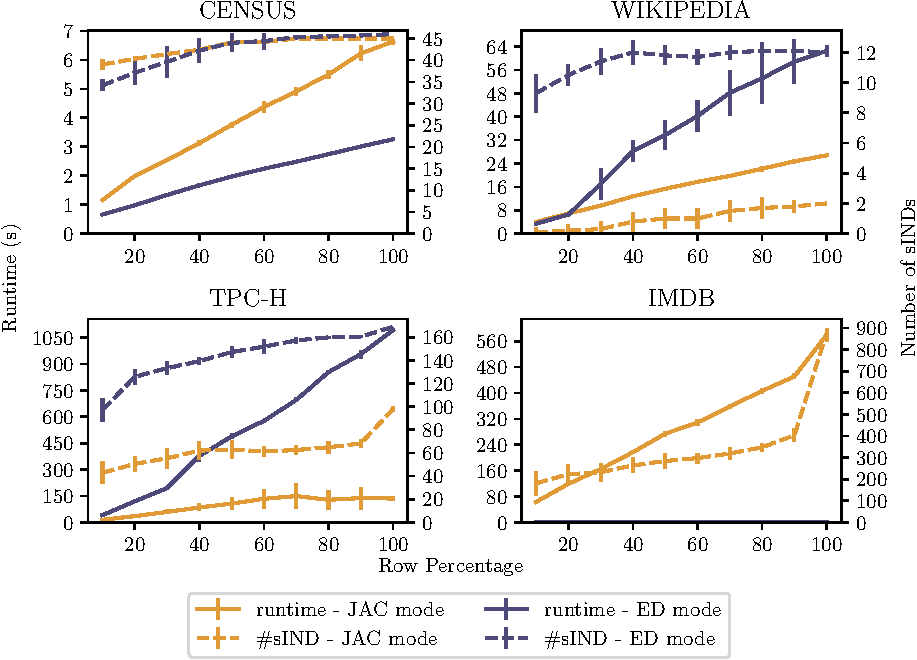
\includegraphics[width=.8\columnwidth]{figures/evaluation/row_scaling-crop.pdf}
    \caption{Row scalability on different datasets (for $ED$ mode $\tau = 1$, for $JAC$ mode $\delta = 0.4$)}
    \label{fig:eval:row}
\end{figure}

\subsubsection{Column Scalability}
%In this section, we want to examine \sawfish's column scalability.
Next, we investigate the scalability of \sawfish with an increasing number of columns.
For this experiment, we randomly sampled column sets for each of the ten column set sizes.
We used 30 samples for each size to accommodate the high variance from different column sets, because the runtime depends on the number of valid sINDs that happen to hold in that sample.
%Similarly to the row scalability experiment, we randomly sampled columns from the input dataset and processed them.
%However, unlike increasing the number of rows, increasing the number of columns does increase the number of sIND candidates.
%Moreover, the runtime of different column combinations varies widely, depending on the number of valid sINDs that happen to hold in that sample.
To explain the variance, we take another look at our introductory example, regarding two sets of two columns each.
Let the first set consist of column \mbox{\emph{results[$\mathtt{name}$]}} and column \mbox{\emph{goalie[$\mathtt{p\_id}$]}}, and the second consist of column \emph{results[$\mathtt{name}$]} and column \emph{goalie[$\mathtt{club}$]}.
As the sIND \emph{results[$\mathtt{name}$]~$\simIND{}$~goalie[$\mathtt{club}$]} as well as the symmetric counterpart are valid, \sawfish needs to iterate through both columns, build indices, and validate all dependent values.
On the other hand, we can already determine after preprocessing that there are no sINDs in the first column set, because of their length difference.
Thus, \sawfish can process it much faster.
We investigate the impact of valid dependencies in Section~\ref{subsection:evaluation:valid_impact}.
%For our experiment, we sample 30 random column sets for each of the ten sample sizes per dataset. % to ensure the validity of our results.
%While in theory, we could try to process all column sets of each sample size, there are too many combinations of a certain size.
%Let $n$ be the total number of columns and $m$ be the size of the column set.
%There are $\binom{n}{m}$ possible $m$-sized column combinations.
%If we want to investigate column sets of size $30$ of the \emph{TPC-H} dataset, there are $\binom{55}{30} = 3.09 \cdot 10^{15}$ different column sets.
%Thus, we look at a fixed number of column sets and still observe differences with increasing column counts.
To emphasize the variance between the results, we present boxplots for each sample size.
Figure~\ref{fig:eval:column_ED} shows the results for the column scalability of the \emph{CENSUS}, \emph{WIKIPEDIA} and \emph{TPC-H} datasets in $ED$ mode.
We omit the \emph{IMDB} dataset for the same reasons as in our row-scaling experiment.
%We sampled ten equidistant data points, starting from column set size~2 and increased the set size by~1 in each step.
%Additionally, we processed the entire dataset of 11 columns.
%Moreover, the variance for column set size 10 is also smaller, because there are only 11 sets to sample, since $\binom{11}{10} = 11$.
%
%\begin{figure}[ht]
%      \centering
%        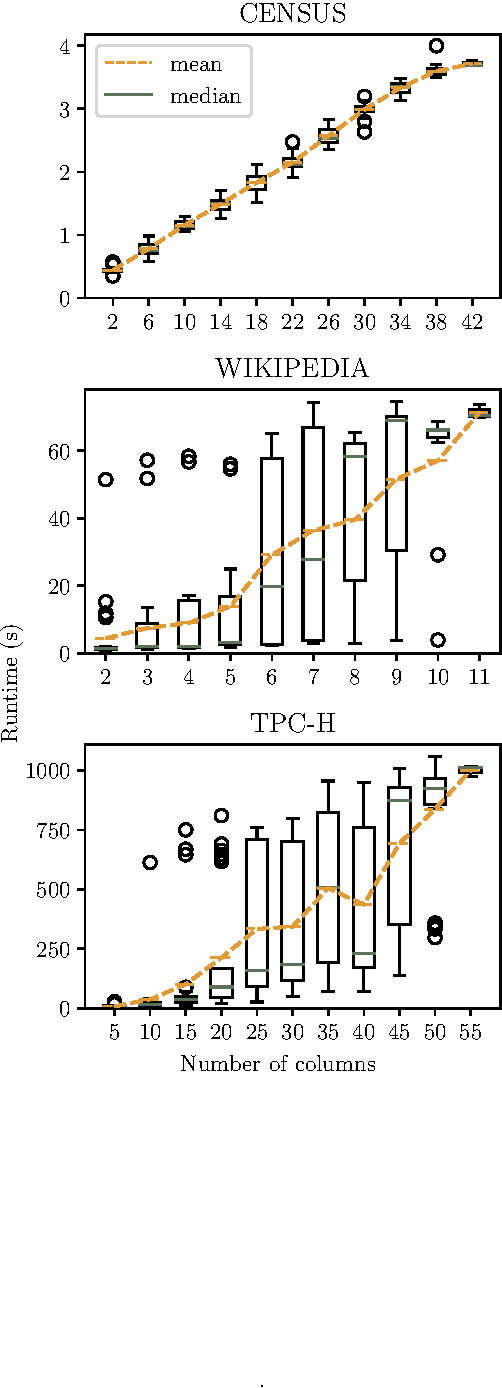
\includegraphics[width=\columnwidth]{figures/evaluation/column_scalingED}
%    \caption{Column scaling}
%    \label{fig:eval:columnScalling}
%\end{figure}

Since the number of sIND candidates grows quadratically in the number of columns, one could expect a quadratic scaling.
However, we observe a linear scaling.
In our experimental setup of sampling from an input dataset, the number of valid sIND candidates on average grows linearly with the number of columns.
%Thus, we do not see a quadratic increase in runtime.
Additionally, we find that \sawfish's runtime in general does not grow over-proportionally with rising data amounts.
This shows the effectiveness of \sawfish's memory handling.

While the \emph{CENSUS} dataset shows almost no variance due to its small size, the runtimes vary widely for the \emph{WIKIPEDIA} and the \emph{TPC-H} dataset.
For the \emph{WIKIPEDIA} dataset, we observe a small runtime variance for column sets of sizes 10 and 11, as only a few sets have such column counts.
The remaining variance can be attributed to the differences between the three experiment runs.
However, we observe some outliers.
On the one hand, there are two outliers for column set size 10 that have a drastically reduced runtime.
On the other hand, there are two outliers for column set sizes 3 to 5 that have a drastically increased runtime.
For column set size 2, there are also a few outliers.
These are artifacts related to the difference between processing a valid sIND and quickly discarding an invalid candidate, as we explained before.
However, they are also related to the dataset ``shape''.
%This is especially visible for the heavy outliers for column set sizes 2 and 10.
The \emph{WIKIPEDIA} dataset consists of two tables:
Table~1 is wider, while Table~2 is longer.
There exists the valid sIND \emph{Table1[$\mathtt{column9}$]} $\simIND{}$ \emph{Table2[$\mathtt{column1}$]}.
It takes roughly 40~seconds to validate this sIND alone, explaining the extreme outlier for column set size~2.
This sIND is also responsible for the two outliers for column set size~10.
There are similar explanations for the other outliers.
%There are three other columns that depend on \emph{Table2[column1]}, too.
%Thus, if the column set misses \emph{Table2[column1]}, the runtime is drastically reduced.
%Moreover, if the column set misses \emph{Table1[column9]}, the runtime is also nearly halved.
%This reduction shows how single sIND candidates can dominate the runtime of the entire algorithm.

When using $JAC$ as similarity measure, the results in Figure~\ref{fig:eval:column_JAC} for the \emph{WIKIPEDIA} dataset look quite similar.
While we can process the data faster overall, the scalability differs not much.
We observe similar outliers because they are not specific to the $ED$ mode.

%\begin{figure}[t]
%    \centering
%    \includegraphics[width=\columnwidth]{figures/evaluation/column_scaling_WIKIPEDIA.pdf}
%    \caption{Column scalability experiment on the \emph{WIKIPEDIA} dataset}
%    \label{fig:eval:column_WIKI}
%\end{figure}
%\begin{figure}[t]
%    \centering
%    \includegraphics[width=\columnwidth]{figures/evaluation/column_scaling_TPCH.pdf}
%    \caption{Column scalability experiment on the \emph{TPC-H} dataset}
%    \label{fig:eval:column_TPC}
%\end{figure}
\begin{figure}
    \centering
    \begin{subfigure}[t]{0.4\textwidth}
        \vskip 0pt
        \centering
        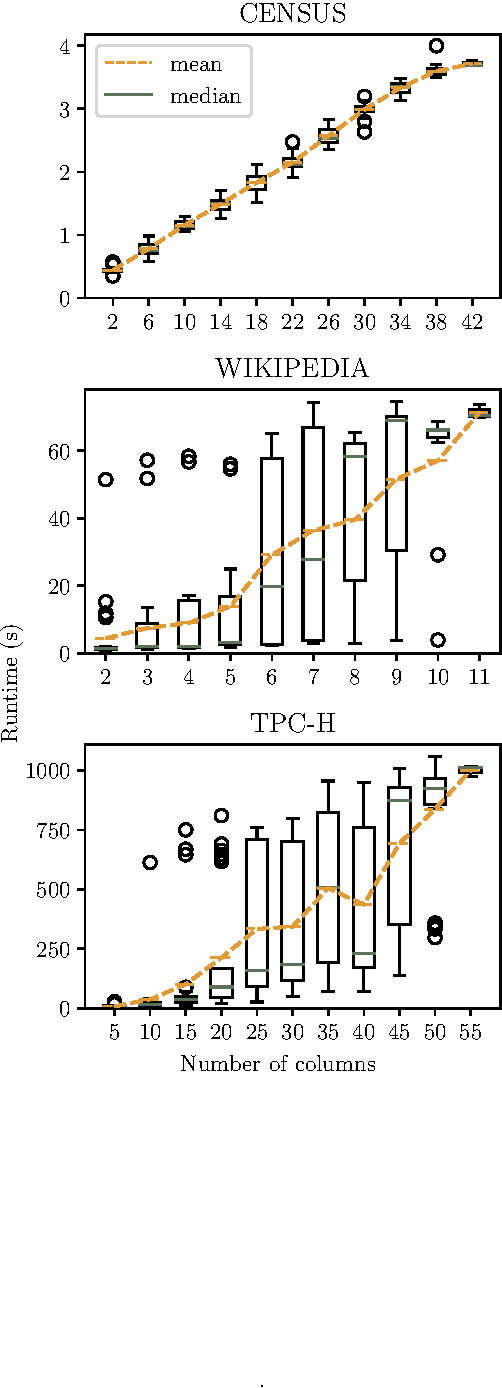
\includegraphics[width=\textwidth]{figures/evaluation/column_scalingED-crop.pdf}
        \caption{$ED$ mode ($\tau = 1$)}
        \label{fig:eval:column_ED}
    \end{subfigure}
    \begin{subfigure}[t]{0.4\textwidth}
        \vskip 0pt
        \centering
        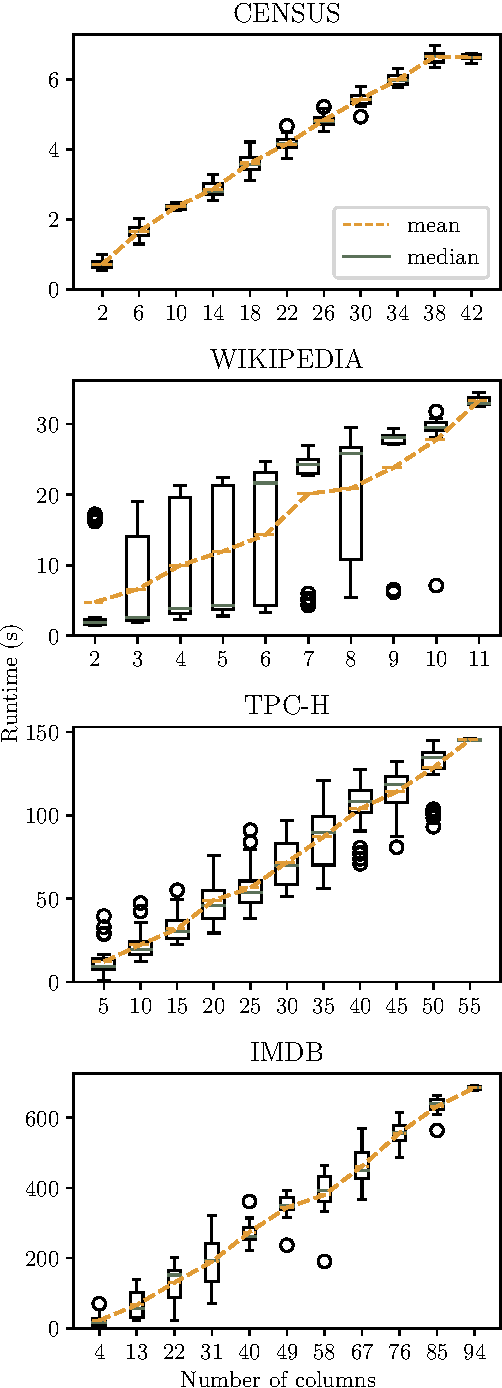
\includegraphics[width=\textwidth]{figures/evaluation/column_scaling_JAC-crop.pdf}
        \caption{$JAC$ mode ($\delta = 0.4$)}
        \label{fig:eval:column_JAC}
    \end{subfigure}
    \caption{Column scalability on different datasets}
    \label{fig:eval:column}
\end{figure}
%\begin{figure*}[ht]
%    \centering
%    \rotatebox{90}{\textbf{\small \hspace{2cm}$ED$ mode ($\tau = 1$)}}
%    \hspace{1cm}
%    \begin{subfigure}[b]{0.35\textwidth}
%        \centering
%        \includegraphics[width=\textwidth]{figures/evaluation/column_scaling_WIKIPEDIA-crop.pdf}
%        \caption{\emph{WIKIPEDIA} dataset}
%        \label{fig:eval:column_WIKI}
%    \end{subfigure}
%    \hspace{2cm}
%    \begin{subfigure}[b]{0.35\textwidth}
%        \centering
%        \includegraphics[width=\textwidth]{figures/evaluation/column_scaling_TPCH-crop.pdf}
%        \caption{\emph{TPC-H} dataset}
%        \label{fig:eval:column_TPC}
%    \end{subfigure}\\
%    \rotatebox{90}{\textbf{\small \hspace{1cm}$JAC$ mode ($\delta = 0.4$)}}
%    \hspace{1cm}
%    \begin{subfigure}[b]{0.35\textwidth}
%        \centering
%       \includegraphics[width=\textwidth]{figures/evaluation/column_scaling_WIKIPEDIA_token-crop.pdf}
%        \caption{\emph{WIKIPEDIA} dataset}
%        \label{fig:eval:column_WIKI_token}
%    \end{subfigure}
%    \hspace{2cm}
%    \begin{subfigure}[b]{0.35\textwidth}
%        \centering
%        \includegraphics[width=\textwidth]{figures/evaluation/column_scaling_TPCH_token-crop.pdf}
%        \caption{\emph{TPC-H} dataset}
%        \label{fig:eval:column_TPC_token}
%    \end{subfigure}
%    \caption{Column scalability on different datasets}
%    \label{fig:eval:column}
%\end{figure*}

For the \emph{TPC-H} dataset, \sawfish's column scaling behaves similarly.
Figure~\ref{fig:eval:column} also shows some outliers in $ED$ mode.
However, these exist for the same reasons, as in the \emph{WIKIPEDIA} dataset.
Similarly to the \emph{WIKIPEDIA} dataset, the general scaling seems to be linear as well.
We observe another artifact of our random sampling: the mean runtime for the column set size 40 is in fact lower than the mean runtime for column set size 35.
Due to the large number of possible column sets of these sizes, such a deviation can occur because of the differences in runtime of individual column combinations.
Interestingly, there seems to be a column set of size 50 that takes longer to process than the entire dataset.
The reason for this result is simply normal measuring deviation.

In comparison to the $ED$ mode, the column scalability on the \emph{TPC-H} dataset in Figure~\ref{fig:eval:column_JAC} in $JAC$ mode presents a near perfect linear scaling of the mean runtime.
We still observe outliers, but the overall variance is lower.
Due to the lower overall runtime, the time spent on processing the input has a larger share of the entire runtime.
Because the input handling is less dependent on specific data characteristics, it differs less than the validation time for equal sample sizes.
Even on the largest \emph{IMDB} dataset, the observed column scaling is linear.
We also observe some outliers that are present for similar reasons as in \emph{WIKIPEDIA} and \emph{TPC-H} datasets.
However, the overall variance compared to the absolute runtime is lower.
This experiment shows that \sawfish's column scaling behavior can be replicated on larger datasets.

\subsubsection{Similarity Measure Thresholds}
\label{subsection:similarity_measure_scalability}
This section examines the impact of the only functional configuration parameter: the similarity threshold.
For the $ED$ mode, this is the number of allowed edits $\tau$.
For the $JAC$ mode, this is the similarity threshold $\delta$.

\paragraph{Edit Distance Threshold}
%
%As we explained in Section~\ref{section:background:problem}, the Levenshtein neighborhood of a string grows exponentially in $\tau$.
%We can observe this phenomenon in our inverted index.
%Due to the higher $\tau$, we segment the string in more parts.
%Thus, each segment consists of fewer characters and its pruning power decreases.
%Therefore, we expect to generate more false positives, which increases the runtime. 
%Increasing $\tau$ also leads to a higher number of simple sINDs, as there are more columns that only contain values, which have $\leq \tau$ characters.
%However, this cannot offset for the larger result set and the increased validation effort.
%
We investigate the edit distance threshold on two datasets:  \emph{CENSUS} and \emph{WIKIPEDIA}.
%Both can be processed with a memory limit of 4~GB, regardless of the edit distance threshold.
We run \sawfish with an edit distance threshold $\tau$ between $0$ and $6$.
We choose 6 as the upper bound, because beyond that threshold a majority of the strings consists of less than $\tau$ characters.
We do not evaluate the other datasets, as they cannot be processed for $\tau = 6$ within our time limit of 24~hours.
Figure~\ref{fig:eval:ed} shows the results for the \emph{CENSUS} dataset.
We plot the runtime and the number of valid sINDs.
While the runtime stays almost constant for lower edit distance thresholds, it quickly rises for $\tau \geq 4$.
%The runtime stays almost constant at around 4~seconds until $\tau = 3$.
%At $\tau = 4$, it roughly doubles to 9~seconds.
%Afterwards, the runtime increases to 12~seconds for $\tau = 5$ and 14~seconds for $\tau = 6$.
%Thus, the runtime more than triples for the observed edit distances.
%However, we cannot observe an exponential increase in runtime.
In contrast, the result set grows over the entire experiment, despite a growing number of simple sINDs (all value lengths are $\leq \tau$).
%\begin{figure}[t]
%    \centering
%    \includegraphics[width=\columnwidth]{figures/evaluation/ed_scaling_CENSUS.pdf}
%    \caption{Edit Distance scaling of the \emph{CENSUS} dataset}
%    \label{fig:eval:ed_CENSUS}
%\end{figure}
%\begin{figure}[t]
%    \centering
%    \includegraphics[width=\columnwidth]{figures/evaluation/ed_scaling_explanation_CENSUS.pdf}
%    \caption{Index Matches for the \emph{CENSUS} dataset with increasing edit distance}
%    \label{fig:eval:ed_explain_CENSUS}
%\end{figure}

\begin{figure}
    \centering
    \begin{subfigure}[b]{.8\textwidth}
        \centering
        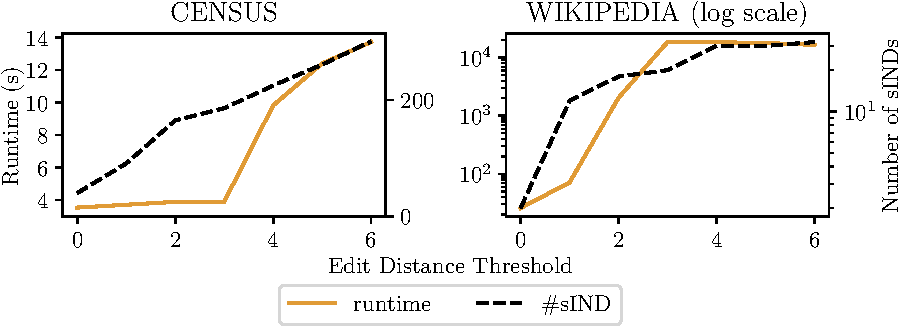
\includegraphics[width=\textwidth]{figures/evaluation/ed_scaling-crop.pdf}
        \caption{Runtime and result set size}
        \label{fig:eval:ed}
    \end{subfigure}
    \begin{subfigure}[b]{.8\textwidth}
        \centering
        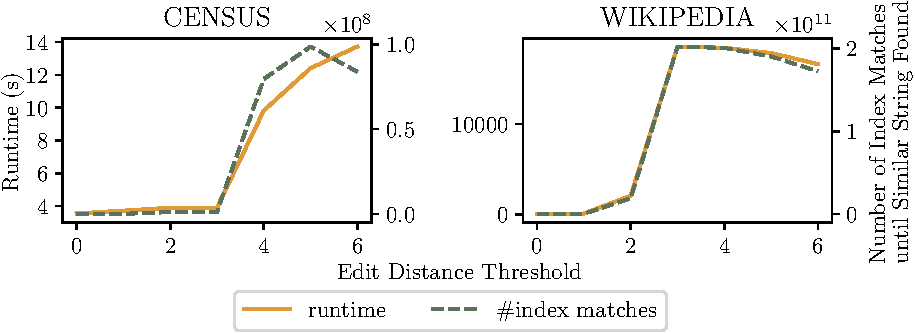
\includegraphics[width=\textwidth]{figures/evaluation/ed_scaling_explanation-crop.pdf}
        \caption{Runtime and index matches until a similar string is found}
        \label{fig:eval:ed_explanation}
    \end{subfigure}
    \caption{Edit distance threshold scaling on different datasets}
\end{figure}

Interestingly, the jump in runtime does not relate to a jump in the result set size.
To investigate the increasing runtime, we look at the number of matches in our index until a similar string was found.
Figure~\ref{fig:eval:ed_explanation} shows the runtime compared to the number of index matches.
We can observe a clear correlation.
There are two factors that influence the number of matches:
the number of dependent values that we need to validate for the candidate sINDs, and the edit distance, which influences the pruning power of the inverted index.
Since the segment length shrinks, there are more coincidental matches.
Both of these factors are dependent on the internal structure of the dataset.
For the \emph{CENSUS} dataset, we observe that there is an increase in coincidental matches for edit distance $\tau \geq 4$ because the number of index matches grows more than the number of discovered sINDs.
For $\tau = 6$, the number of index matches decreases again, because we can validate some strings earlier due to the greater edit distance.
However, the effort for each edit distance computation increases, so overall the runtime still increases.

The results for the \emph{WIKIPEDIA} dataset are on the right-hand side of Figure~\ref{fig:eval:ed}.
As before, we plot the runtime and the number of valid sINDs, here in a logarithmic scale to better show the differences in runtime.
\sawfish's runtime increases significantly for lower edit distance thresholds and reaches it peak at $\tau = 3$.
Afterward, it decreases slightly for larger edit distance thresholds, while the result set size stays almost constant.
%The runtime doubles between $\tau = 0$ at 26 seconds to 65 seconds at $\tau = 1$.
%At $\tau = 2$, it increases to \num{2046} seconds (about 34~minutes).
%\sawfish's runtime peaks at $\tau = 3$ with \num{18570} seconds, i.e., 5~hours and 10~minutes.
%Afterwards, it decreases for $\tau = 4, 5, 6$.
%\sawfish needs around 4~hours and 30~minutes to discover all sINDs with an edit distance threshold $\tau=6$.
%The result set size increases over the entire experiment.
%However, while we observe a plateau for $\tau$ $4 \to 6$, there are jumps for $\tau$ $0 \to 1$ and $3 \to 4$.

To investigate both the stark increase and the following decrease in runtime, we regard the index matches once again.
We use linear scaling in Figure~\ref{fig:eval:ed_explanation} to better visualize the similarity of the lines.
Interestingly, the two curves have a nearly identical shape.
In contrast to the \emph{CENSUS} dataset, the early increase in the number of valid sINDs coincides with the increase in the number of index matches.
Due to the higher number of valid candidates, we have to validate more dependent values.
However, the number of index matches for $\tau = 3$ is significantly higher per dependent value than for all other edit distances.
For each dependent value, we find an average of \num{17000} index matches for $\tau = 3$, while there are only \num{8500} matches on average for $\tau = 4$.
This means that there are many index matches for $\tau = 3$ that cannot be validated.
Thus, we have to iterate the complete list of index matches for each dependent value.
In contrast, we can validate more values for $\tau = 4$, so we do not have to process all index matches.
Additionally, this explains the increase in valid sINDs for $\tau = 4$.
This trend of earlier validation continues for $\tau = 5$ and $\tau = 6$.
It also indicates that the number of coincidental matches does not increase significantly.
As explained for the \emph{CENSUS} dataset, the number of index matches decreases over-proportionally to the decrease in runtime, because each individual edit distance computation takes longer.

%\begin{figure}[t]
%    \centering
%    \includegraphics[width=\columnwidth]{figures/evaluation/ed_scaling_WIKIPEDIA.pdf}
%    \caption{Edit Distance of the \emph{WIKIPEDIA} dataset}
%    \label{fig:eval:ed_WIKIPEDIA}
%\end{figure}
%
%\begin{figure}[t]
%    \centering
%    \includegraphics[width=\columnwidth]{figures/evaluation/ed_scaling_explanation_WIKIPEDIA.pdf}
%    \caption{Index Matches for the \emph{WIKIPEDIA} dataset with increasing edit distance}
%    \label{fig:eval:ed_explain_WIKIPEDIA}
%\end{figure}

In conclusion, \sawfish is able to discover sINDs also for higher edit distance thresholds.
However, the runtime is dependent on the internal structure of the dataset, namely the number of valid sINDs and the number of coincidental index matches.

\paragraph{Jaccard Similarity Threshold}
We investigate the effect of different similarity thresholds $\delta$ on the \emph{TPC-H} dataset.
We focus on this dataset, because it contains strings with varying token counts; thus the difference for different thresholds is more noticeable.

Figure~\ref{fig:eval:jac_sim_scalability} shows the runtime and the result set size for different $\delta$, ranging from $0.1$ to $1.0$.
%Interestingly, the runtime spikes for $\delta = 0.2$ and $\delta = 0.3$.
%This spike is not correlated to the drop in the number of found sINDs between $\delta = 0.5 \to 0.6$, but rather related.
The reason for the drop in sINDs between $\delta = 0.5 \to 0.6$ is the content of the discovered sINDs.
For $\delta \leq 0.5$, we find matches between single token and two token strings that form the extra sINDs.
%However, these matches are no longer valid for $delta > 0.5$.

The runtime behavior is related to the validation characteristics, especially for values with more tokens.
For $\delta = 0.1$, for every string we need at most two matching tokens to validate the similarity, because we limit the number of tokens to 10.
For $\delta = 0.2$ and $\delta = 0.3$, we cannot validate each string so easily, but the threshold is still low.
Thus, many coincidental matches occur, which slow down the discovery process.
For $\delta \geq 0.4$, the number of coincidental matches decreases, but the validation effort for each individual value grows, because we need to find more matching tokens.
Nonetheless, the runtime converges.
This behavior is different from the edit distance case, because we discover fewer sINDs overall, but also the number of coincidental matches is lower.
\begin{figure}[ht]
    \centering
    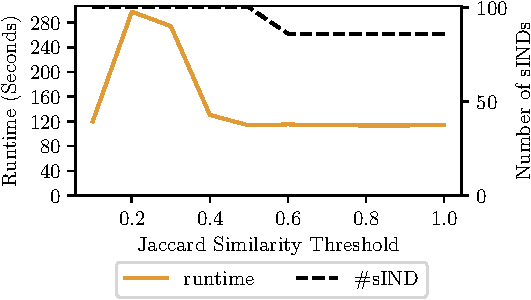
\includegraphics[width=.55\textwidth]{figures/evaluation/sim_scaling_TPCH_token-crop.pdf}
    \caption{Jaccard similarity scalability on the \emph{TPC-H} dataset}
    \label{fig:eval:jac_sim_scalability}
\end{figure}

\subsection{Impact of Valid Dependencies}
\label{subsection:evaluation:valid_impact}
The column scalability experiment illustrated how much of the overall runtime depends on individual columns or even individual sIND candidates.
Thus, we explore this effect in more detail.
Valid dependencies contribute to the runtime especially, because we need to validate each dependent value and cannot abort early.

Figure~\ref{fig:eval:valid_dependencies} shows the runtime for each potential sIND candidate in \emph{CENSUS}, \emph{WIKIPEDIA} and \emph{TPC-H} datasets.
For clarity, we only show the results of $ED$ mode, but the findings are similar for the $JAC$ mode.
We highlight valid candidates and order the candidates by the number of distinct dependent values.
As usual, we filtered any candidates that were discarded during preprocessing.
\begin{figure}[ht]
    \centering
    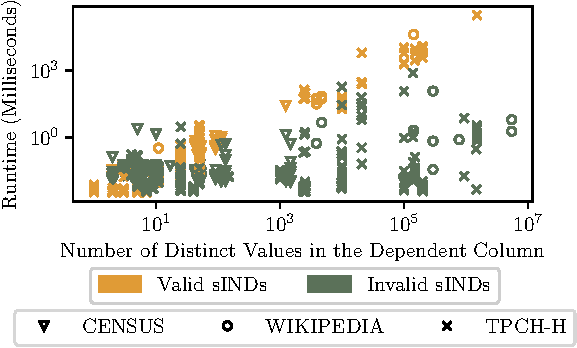
\includegraphics[width=0.6\textwidth]{figures/evaluation/valid_sIND_impact-crop.pdf}
    \caption{Difference in runtime of valid and invalid candidate validation (log-scale for both axes)}
    \label{fig:eval:valid_dependencies}
\end{figure}

We can observe two expected phenomena.
Larger dependent columns and valid dependencies need more time to validate.
The scaling behavior is more interesting.
While the runtime for valid dependencies continuously increases for larger dependent columns, the scaling is not clear for invalid dependencies.
This is because \sawfish needs to find a dependent value for which no similar referenced value exists.
%Since the candidates passed the preprocessing filter, they might form a valid sIND.
Therefore, the runtime for invalid dependencies is dependent on the position of the counterexample in the dependent column and thus almost random.
This behavior can be observed especially for larger invalid dependencies, where the position differences between counterexamples are more noticeable.

\subsection{Comparison to Related Work}

%This section compares \sawfish to the competitors that we introduced above.
%We use all datasets to compare the three different approaches.
The experiments in this section compare \sawfish with the baselines using all datasets.
%For every dataset, we use a memory limit of 4~GB.
%For the \emph{IMDB} dataset, we used 32~GB as a memory limit, so all algorithms can process it.
%, which is about 2x the size of our largest dataset. 
%Since the baseline needs to operate entirely in main memory, we need to set a high memory limit.
%Still, the baseline was not able to process the \emph{IMDB} dataset within these memory requirements, so we exclude it from the evaluation of this dataset.

\paragraph{Edit Distance Mode}
%First, we evaluate the different algorithms when choosing the edit distance as similarity measure.
The following experiment compares the runtimes for an edit distance threshold $\tau = 0$. In this setting, all performance results are comparable since all algorithms discover traditional INDs.
The left-hand side of Figure~\ref{fig:eval:comparsion_ed} shows the results for all datasets, scaled per dataset to the longest running algorithm.
Interestingly, for the CENSUS dataset, our naive baseline is the fastest algorithm, while \algorithmName{Binder} needs the most time to complete the search.
Since the dataset is relatively small, the benefit of \sawfish's preprocessing does not outweigh its overhead.
Nonetheless, \sawfish is relatively close to the runtime of the baseline.

\begin{figure*}[ht]
    \centering
    \begin{subfigure}[b]{\textwidth}
        \centering
        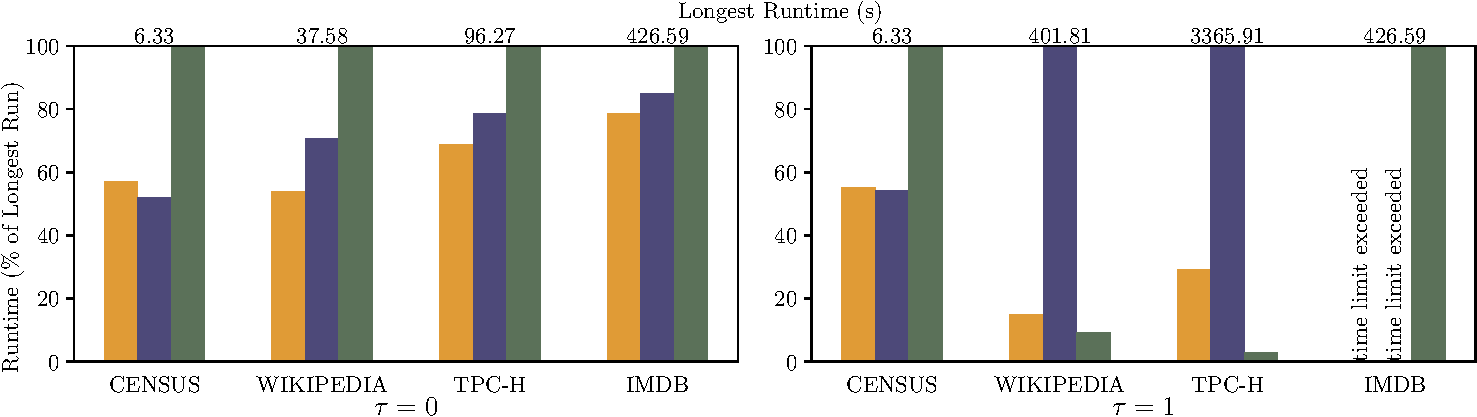
\includegraphics[width=\textwidth]{figures/evaluation/competitor_bars-crop.pdf}
        \caption{$ED$ mode}
        \label{fig:eval:comparsion_ed}
    \end{subfigure}\\
    \begin{subfigure}[b]{\textwidth}
        \centering
        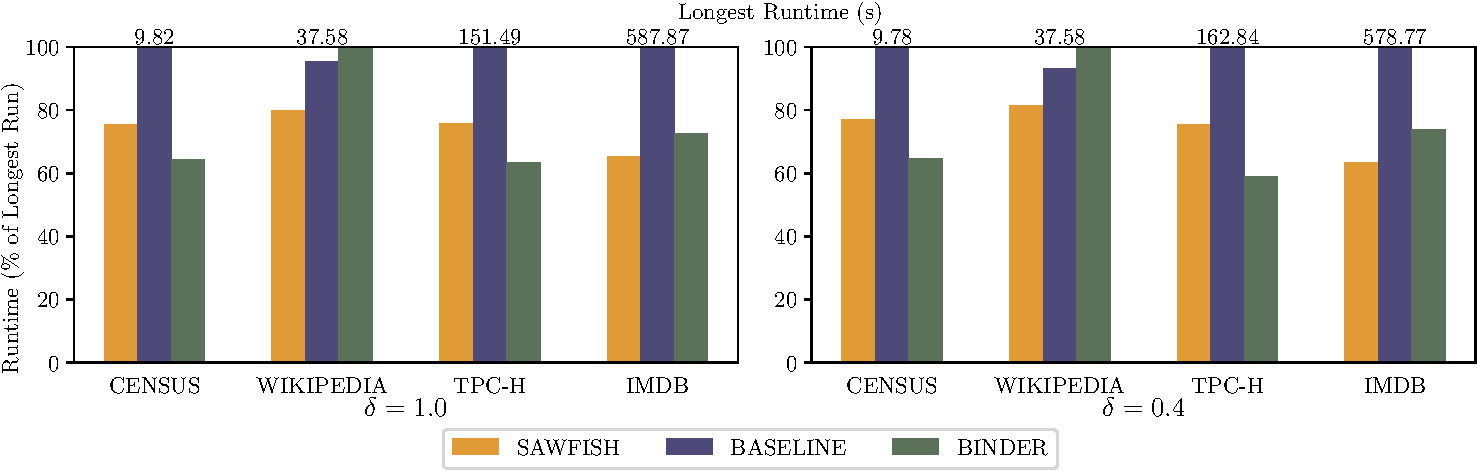
\includegraphics[width=\textwidth]{figures/evaluation/competitor_bars_token-crop.pdf}
        \caption{$JAC$ mode}
        \label{fig:eval:comparison_jac}
    \end{subfigure}
    \caption{Comparison of \sawfish to related work}
\end{figure*}

For the \emph{WIKIPEDIA}, the \emph{TPC-H} and the \emph{IMDB} datasets, \sawfish's preprocessing combined with the improved index access pattern improves the performance over the baseline.
\algorithmName{Binder} is the slowest in this experiment, because the two other algorithms can operate entirely in main memory if the entire dataset fits.
\algorithmName{Binder} eagerly writes every bucket to disk after preprocessing, because it anticipates larger dataset sizes. % and decreases implementation complexity by always writing to disk.
%The results of the \emph{IMDB} dataset show \algorithmName{Binder}'s specialization in discovering traditional INDs from large datasets.
%\sawfish's runtime is more than twice that of \algorithmName{Binder}.
%In particular, this shows the effectiveness of \algorithmName{Binder}'s approach for discovering INDs, e.g., discovering multiple INDs at once, as explained in Section~\ref{section:related_work2}. The baseline 
%cannot process the dataset, because it exceeds our memory limit.

Next, we set $\tau=1$, i.e., allow sINDs with an edit distance of up to 1 for each value.
We present them on the right-hand side of Figure~~\ref{fig:eval:comparsion_ed}.
The results for \algorithmName{Binder} remain in the figures for comparison purposes, even though \algorithmName{Binder} cannot discover such dependencies.
The result for the \emph{CENSUS} dataset is comparable in runtime to the IND discovery experiment.
However, the results for the \emph{WIKIPEDIA} dataset and the \emph{TPC-H} dataset show the superiority of \sawfish.
For the \emph{TPC-H} dataset, we observe the higher complexity of the sIND discovery compared to the IND discovery.
The runtime of \sawfish is about one third of the baseline's runtime.
This visualizes the improvements that we accomplish by modifying \algorithmName{PassJoin}'s approach.
The effect is even larger in the \emph{WIKIPEDIA} dataset:
\sawfish outperforms the baseline by a factor of around~6.5. 
%and is in fact close to the runtime of \algorithmName{Binder}.
\sawfish was not able to discover all sINDs for the \emph{IMDB} dataset, as it exceeded the time limit of 24~hours.
This emphasizes the difficulty of sIND discovery, because \sawfish discovered all INDs (without allowing similarity) in around 6~minutes.
We discuss ideas to improve the validation speed in Section~\ref{section:discussion}.

Our results show that \sawfish can efficiently discover sINDs for reasonably large datasets.
While the sIND discovery is a hard problem, \sawfish manages to process some datasets in a comparable time to the IND discovery.
For all larger datasets, \sawfish outperforms the baseline.
%However, we also observe \sawfish's weaknesses in the \emph{IMDB} dataset.

\paragraph{Jaccard Similarity Mode}
%Second, we compare the runtime of \sawfish when choosing the Jaccard similarity as similarity measure.
%Figure~\ref{fig:eval:comparison_jac} shows the results for all four datasets for $\delta = 1.0$ on the left-hand side.
Figure~\ref{fig:eval:comparison_jac} shows the results for $\delta = 1.0$ on the left-hand side.
%Thus, all algorithms discover the same traditional INDs.
\algorithmName{Binder} performs best for the \emph{CENSUS} and the \emph{TPC-H} datasets, while \sawfish performs best on the other two datasets, \emph{WIKIPEDIA} and \emph{IMDB}.
Besides \algorithmName{Binder}'s algorithmic advantages, the overhead for tokenization inhibits the performance of the other two algorithms.
While \sawfish and the baseline could have found more dependencies due to the order insensitivity of the Jaccard similarity, we did not observe such effects in our dataset.
Nonetheless, they have to tokenize each value.
On the other hand, \sawfish and the baseline can once again operate entirely in main memory.
Therefore, they gain an advantage in datasets that do not create many tokens per value, e.g., \emph{WIKIPEDIA} and \emph{IMDB}.
%Thus, \sawfish performs best on these datasets.

For the next experiment, we set $\delta = 0.4$ and show the results on the right-hand side of Figure~\ref{fig:eval:comparison_jac}.
%This parameter change does not result in different performance characteristics.
%This parameter change does not change the general performance characteristics.
In general, the performance characteristics remain similar.
The gap between \sawfish and \algorithmName{Binder} widens a bit for the \emph{TPC-H} dataset, while it closes a bit for the \emph{WIKIPEDIA} dataset. 
For the \emph{IMDB} dataset, \sawfish and the baseline improve their runtime, because they can validate string pairs of traditional INDs earlier due to the lower threshold.

When using the Jaccard similarity, \sawfish can discover sINDs in a time that is comparable to the state-of-the-art IND discovery algorithm \algorithmName{Binder}.
We also show that \sawfish outperforms a baseline for all datasets.

\subsection{Joinability Case Study}
In this experiment, we want to investigate whether the discovered similarity inclusion dependencies can indeed indicate joinability in the presence of typos or other data errors.
Joinability means that two columns can be linked together because they contain similar data from the same domain\cite{chia2019hyperloglog}.
To investigate the performance on a more heterogeneous data source, we ran \sawfish on a subset of the \emph{2015 Web Table Corpus (WTC)}\cite{lehmberg2016corpus}.
This corpus consists of automatically crawled web tables.
While these web tables are typically smaller than traditional database tables, more web tables are usually processed simultaneously.
Our experiment uses an edit distance threshold $\tau = 1$ and the random sample of \num{10000} tables from the original source\footnote{\url{http://data.dws.informatik.uni-mannheim.de/webtables/2015-07/sample.gz}}.
However, we process only the \num{2516} relational tables in that set.
We omit numeric columns to visualize the results better.
\sawfish runs in $ED$ mode, because we find more and also more interesting results.

In total, we observe \num{1044} sINDs that consist only of strings and are not traditional INDs, i.e., the dependent column contains at least one value for which only a similar value can be found in the referenced column.
%Some of these sINDs are purely coincidental.

We manually annotated the sINDs to assess their genuineness.
Overall, we found 161~(15\%) meaningful sINDs, while 671~(64\%) sINDs are coincidental.
Coincidental sINDs are dependencies where the two columns contain data from different domains, but the values happen to be similar purely by chance. 
For example, we discover an sIND between the cost column of a university audiobook chapter list and the first name column of a table of probate files.
Since it is a university audiobook, all chapters are ``\data{Free}''.
Thus, the entire value set of the column contains only this value.
In turn, in the probate file table, we find the first name \data{Fred}.
The remaining 212~(20\%) sINDs are caused by errors in the header detection of the underlying dataset.

Additionally, we investigated the \emph{characteristics} of meaningful and coincidental sINDs.
For our example dataset, we observe that there are two criteria that reduce the number of coincidental sINDs significantly.
First, the maximum number of characters of any value of the dependent side is above three.
Second, the portion of dependent values that match only similarly to a value on the referenced side is below 30\%.
Given these two filters, the number of coincidental sINDs is reduced by 638 to 33~(20\%). 
The number of meaningful sINDs that fulfill these criteria is 101~(64\%).
%Therefore, we discover this sIND.

%Nevertheless, we also discover meaningful sINDs.
To exemplify the discovered sINDs, we showcase some meaningful sINDs.
For example, there is an sIND between the data type column of an API description and the data type column of the input parameters of a program.
While, one column uses the uppercase versions, such as \data{Float} and \data{String}, the other column uses the lowercase versions, such as \data{float} and \data{string}.
Despite these columns obviously containing data of the same domain, they do not form a traditional IND.
Nonetheless, they could be joined to investigate usages for the same data type.

We present another example of a meaningful sIND in Table~\ref{table:eval:best_matches}.
There are multiple tables inside the sample that contain data about college athletes.
Typically, students are classified into four categories: freshman, sophomore, junior, and senior -- multiple columns contain abbreviations of these categories.
However, as the table shows, they do not match perfectly, so they do not form a traditional IND.
%The Virginia Commonwealth University (VCU) uses an uppercase first letter, followed by a lower case letter.
%By contrast, the CFB stats for the Tulsa Golden Hurricane (CFB) use uppercase letters only.
%The last variation of the NCAA Baseball stats (NCAA) is to append a point to the VCU style abbreviations.
Interestingly, we only discover the sINDs \mbox{\emph{VCU} $\simIND{}$ \emph{CFB}} and \mbox{\emph{VCU} $\simIND{}$ \emph{NCAA}} (and their symmetric partners).
To also discover \mbox{\emph{CFB} $\simIND{}$ \emph{NCAA}}, we need to increase the edit distance threshold to~2.
Nevertheless, all of this data belongs to the same domain.
Moreover, if we want to compare students from the same category, it makes sense to join these values.
\begin{table}[h]
\centering \small
\caption{Example sINDs in the \emph{WTC} dataset}
\label{table:eval:best_matches}
\begin{tabular}{@{}lll@{}}
\toprule
VCU Football	& CFB: Tulsa Golden Hurricane	& NCAA Baseball \\
\midrule
Fr 				& FR       						& Fr.     		\\
So      		& SO                            & So.     		\\
Jr    			& JR          					& Jr.     		\\
Sr    			& SR          					& Sr.    		\\
\bottomrule
\end{tabular}
\end{table}
% While many sINDs within the \emph{WTC} were coincidental, there also are multiple valid examples.
% These show the benefits of allowing similar values, because otherwise these dependencies would go unnoticed.
% Furthermore, we have to consider that this experiment is conducted on a subset of 200 million web tables.
% If \sawfish ran on a more homogenous dataset, we expect a lower number of random sINDs.
% Nevertheless, we could show that our results can indeed indicate joinability.
\section{Conclusion}
\label{section:discussion}

This work introduces the formal concept of similarity inclusion dependencies (sINDs), extending traditional inclusion dependencies with a similarity measure.
%Thus, they allow for data errors and uncover hidden dependencies.
%Additionally, we present \sawfish, the first approach to efficiently discover such sINDs in a given dataset.
%Moreover, we investigate \sawfish's performance characteristics for a wide set of parameters and datasets.
%This section summarizes the main insights and discusses the current limitations of \sawfish.
%\subsection{Conclusion}
%In this work, we investigated multiple aspects of sINDs.
%First, we identified use cases for sINDs.
%These included the use cases of traditional INDs, such as foreign-key candidate and join partner discovery.
First, we identified use cases for sINDs, which include discovering foreign-key candidates and join partners.
%Additionally, sINDs can be used to determine erroneous data sources within a large data management system.
Second, we formalized an sIND definition that extends traditional INDs with an arbitrary similarity measure.
Third, we presented \sawfish, the first efficient approach to automatically discover sINDs from data.
It finds all unary sINDs based on the edit-distance and the Jaccard similarity measure.
\sawfish combines approaches of traditional IND discovery and string similarity joins with a novel sliding-window approach and lazy candidate validation. %discovering unary sINDs based on the edit-distance similarity measure.
Fourth, we evaluated \sawfish, showing that it scales well in the number of rows, and in the number of columns.
%Furthermore, we observed that \sawfish does not require more main memory than the size of the largest column to run efficiently.
%However, we also discovered some limitations that we address in the next section.
Compared to a baseline implementation, we outperformed it by a factor of up to~6.5.
Finally, we examined the sINDs discovered by \sawfish and observed real-world examples indicating joinability.

%\subsection{Limitations and Future Work}
%\label{section:discussion:future}
%While \sawfish can discover sINDs efficiently, it relies on certain assumptions.
%These include the requirement that each column must fit entirely into main memory.
%In the future, this might be avoided with better locality sensitive hashing techniques, so the bucketing process can adopt the hash-partitioning scheme of \algorithmName{Binder}.
%Thus, there would be no need for a main memory requirement.
%However, since \sawfish needs to fit only a single column into main memory, the real-world impact of this constraint is limited.
%
%Another limiting aspect of \sawfish is its runtime on larger datasets and higher edit distances.
While sIND discovery is a harder problem than traditional IND discovery, the runtime could be further improved by multithreading or distributing the process.
As \algorithmName{Sindy}~\cite{dursch2019eval} demonstrated, distribution can significantly improve the performance.
However, we observed that a single column or even a single sIND candidate can dominate the runtime.
Therefore, it is not trivial to scale \sawfish's approach to multiple threads or nodes.
Further future work shall extend \sawfish to discover n-ary sINDs.% and to use similarity measures beyond the edit distance.
%
% Besides the execution characteristics, \sawfish's results are also limited in some aspects.
% First, \sawfish can discover only unary sINDs.
% However, the sIND definition also allows for n-ary sINDs.
% Thus, \sawfish can be extended to discover n-ary sINDs, too.
% This massively increases the search space, since we would need to process not only pairs of columns, but rather pairs of column lists that can form an sIND.
% Therefore, this could be combined with faster validation algorithms to keep the execution time reasonable.
%
%Second, \sawfish supports only the edit distance as a similarity measure. 
%While this is a good starting point, there are certainly other interesting similarity measures.
%To work with other edit-based similarity measures, large parts of \sawfish can be reused.
%For example, the deduplication and the length splitting of the preprocessing are helpful for all edit-based similarity measures.
%Additionally, we can define tighter pruning rules for other measures.
%For example, the Hamming distance is defined only on similar sized strings, so we could improve our length pruning~\cite{hamming1950error}.

% Our index in the main discovery step is specialized on the edit distance, so it would need to be adapted for other similarity measures.
% Moreover, to use token-based similarity measures, there would be more necessary changes.
% The preprocessing would need to split the input values into tokens and perform pruning by their token count.
% The main discovery implementation needs to be modified for the selected similarity measure.
% However, the general structure of \sawfish could be applied.
% This includes preprocessing the input data, generating sIND candidates, and validating the candidates.
% \sawfish includes easily adaptable functions that reliably complete the tasks.

% There might be more opportunities in the future to extend traditional data dependencies with similarity measures.
% In this regard, \sawfish provides a foundation that can be used for further ideas.
%\balance

%%
%% The acknowledgments section is defined using the "acks" environment
%% (and NOT an unnumbered section). This ensures the proper
%% identification of the section in the article metadata, and the
%% consistent spelling of the heading.
%\begin{acks}
%To Robert, for the bagels and explaining CMYK and color spaces.
%\end{acks}

%%
%% The next two lines define the bibliography style to be used, and
%% the bibliography file.
%\bibliographystyle{ACM-Reference-Format}
%\bibliography{sample-base}
\printbibliography

\end{document}
\endinput
%%
%% End of file `sample-authordraft.tex'.
